% PUSIM.tex -- Pileup in the CMS Phase-2 simulation: the signal, the pileup, and the two together.
% Chapter of the JitJet book (JitJetSW/Journey). Compile with
%     pdflatex PUSIM.tex && pdflatex PUSIM.tex
% from this directory; the figures are read from ../../test/PU_Phase2/ (runPileup_mcPhase2_BBbar.sh output).
\documentclass[11pt,a4paper]{article}

\usepackage[T1]{fontenc}
\usepackage[utf8]{inputenc}
\usepackage{lmodern}
\usepackage{textcomp}
\usepackage{microtype}
\usepackage[a4paper,margin=22mm,top=24mm,bottom=26mm]{geometry}
\usepackage{amsmath,amssymb}
\usepackage{graphicx}
\usepackage{xcolor}
\usepackage{booktabs}
\usepackage{multirow}
\usepackage{array}
\usepackage{tabularx}
\usepackage{caption}
\usepackage{subcaption}
\usepackage{float}
\usepackage{placeins}
\usepackage{enumitem}
\usepackage{listings}
\usepackage{tikz}
\usetikzlibrary{arrows.meta,positioning,shapes.geometric,fit,calc}
\usepackage{fancyhdr}
\usepackage{url}
\urlstyle{tt}
\usepackage[colorlinks=true,linkcolor=blue!50!black,citecolor=blue!50!black,urlcolor=blue!50!black]{hyperref}

\graphicspath{{../../test/PU_Phase2/}}

% ---------------------------------------------------------------- colours of the pages (SimHitAnalyzer kKindColor)
\definecolor{puearly}{RGB}{178,160,0}     % ROOT kYellow+2
\definecolor{puintime}{RGB}{102,153,255}  % ROOT kAzure-4
\definecolor{pulate}{RGB}{255,120,120}    % ROOT kRed-7
\definecolor{sigchg}{RGB}{0,0,0}
\definecolor{signeu}{RGB}{153,0,153}
\definecolor{sigpho}{RGB}{0,153,0}
\definecolor{codebg}{RGB}{245,245,245}

\lstset{
  basicstyle=\ttfamily\footnotesize,
  backgroundcolor=\color{codebg},
  frame=single, framerule=0pt, framesep=4pt,
  breaklines=true, breakatwhitespace=false,
  columns=fullflexible, keepspaces=true,
  showstringspaces=false,
  xleftmargin=4pt, xrightmargin=4pt,
  aboveskip=6pt, belowskip=6pt,
}
\lstdefinestyle{py}{language=Python, keywordstyle=\color{blue!60!black}, commentstyle=\color{gray}, stringstyle=\color{green!40!black}}
\lstdefinestyle{sh}{language=bash, keywordstyle=\color{black}, commentstyle=\color{gray}}
\lstdefinestyle{cpp}{language=C++, keywordstyle=\color{blue!60!black}, commentstyle=\color{gray}}

\newcommand{\code}[1]{\texttt{#1}}
\newcommand{\pt}{\ensuremath{p_{\mathrm{T}}}}
\newcommand{\bx}{\ensuremath{\mathrm{bx}}}
\newcommand{\bbbar}{\ensuremath{b\bar{b}}}
\newcommand{\GeV}{\,\mathrm{GeV}}
\newcommand{\ns}{\,\mathrm{ns}}
\newcommand{\cm}{\,\mathrm{cm}}
\newcommand{\mb}{\,\mathrm{mb}}
\newcommand{\sigin}{\ensuremath{\sigma_{\mathrm{inel}}}}
\newcommand{\ptHat}{\ensuremath{\hat{p}_{\mathrm{T}}}}

% ---------------------------------------------------------------- "in plain words" boxes for first-time readers
% (tcolorbox / mdframed are not in this TeX Live; a saved minipage in an \fcolorbox does the job, so keep
% the boxes shorter than a page: they do not break across pages)
\definecolor{plainbg}{RGB}{240,246,255}
\definecolor{plainrule}{RGB}{60,100,170}
\newsavebox{\plainbox}
\newenvironment{plainwords}[1][In plain words]{%
  \par\medskip\noindent\setlength{\fboxsep}{6pt}\setlength{\fboxrule}{0.6pt}%
  \begin{lrbox}{\plainbox}\begin{minipage}{\dimexpr\textwidth-2\fboxsep-2\fboxrule\relax}\small
  \textbf{\textcolor{plainrule}{#1.}}\ \ignorespaces}{%
  \end{minipage}\end{lrbox}\noindent\fcolorbox{plainrule}{plainbg}{\usebox{\plainbox}}\par\medskip}

\captionsetup{font=small,labelfont=bf,width=0.95\textwidth}
\setlist{nosep,leftmargin=*}
\emergencystretch=1.5em

\pagestyle{fancy}
\fancyhf{}
\fancyhead[L]{\small JitJet book -- Pileup in the Phase-2 simulation}
\fancyhead[R]{\small\thepage}
\renewcommand{\headrulewidth}{0.3pt}

\title{\textbf{Pileup in the CMS Phase-2 simulation}\\[4pt]
  \large The signal, the pileup, and the two together: from the minimum-bias library\\
  to the \code{MixingModule} and the \code{CrossingFrame}s, drawn with \code{SimHitAnalyzer}}
\author{JitJet book, \code{JitJetSW/Journey} -- \code{doc/pu/PUSIM.tex}}
\date{CMSSW\_15\_0\_5, Phase-2 detector D110, 14\,TeV; results of \code{test/PU\_Phase2/}, 26 October 2026}

\begin{document}
\maketitle

\begin{abstract}
\noindent
This chapter follows the same event as the SIM chapters of the book (run~1, lumi~1, event~1 of the Phase-2
\bbbar{} sample, $\ptHat > 100\GeV$) one step further: into the DIGI step, where the minimum-bias collisions of
the same and of the neighbouring bunch crossings are added to it. It explains what pileup is and why the HL-LHC
has about 200 collisions per bunch crossing, how CMSSW builds a pileup library and mixes it into the signal
with the \code{MixingModule}, what the mixed event looks like to the digitisers (\code{CrossingFrame}s, event
ids, time offsets), how the truth survives the mixing (\code{PileupSummaryInfo}, \code{TrackingParticle}s,
\code{CaloParticle}s), and what all of this does to the SimHits of one event, station by station, on three
samples drawn with the same \code{SimHitAnalyzer} pages: (a) the signal alone, (b) one minimum-bias event
of the library alone, and (a+b) the signal with 18 mixed pileup events, in-time and out-of-time. The last
sections scale the numbers to the production scenario ($\mathrm{PU}=200$, bunch crossings $-3\ldots3$) and
list how to reproduce and extend the exercise with \code{runPileup\_mcPhase2\_BBbar.sh}.
The chapter is written for a student who meets pileup for the first time: the boxes marked ``In plain
words'' restate each key idea without the CMSSW vocabulary, section~\ref{sec:before} collects the
conventions, and the questions at the end of section~\ref{sec:samples} check the understanding. A reader in a
hurry can read the boxes, the tables and the figure captions first.
\end{abstract}
\clearpage
\tableofcontents
\clearpage

% ======================================================================================================
\section{Before you start}
\label{sec:before}

This chapter is written for a student who has followed the SIM chapters of the book and now meets pileup for
the first time. Nothing in it needs more than that, but it uses a handful of words and conventions on every
page, and it helps to have them in one place before the first figure.

\paragraph{What you should already know.} From the GEN and SIM chapters: that a generator (Pythia8) produces
the particles of one proton--proton collision and hands the stable ones (the \emph{primaries}) to Geant4;
that Geant4 transports them through the detector and leaves \emph{SimHits} where they cross a sensitive
volume (a \code{PSimHit} in a tracker or muon sensor, a \code{PCaloHit} in a calorimeter cell), together with
the \code{SimTrack}s and \code{SimVertex}s that record which particle produced which; and how a
\code{SimHitAnalyzer} page is read (one station per page, three views, colour = kind of the signal primary
the hit descends from). If any of these is unfamiliar, the SIM chapter (\code{doc/sim/At<station>.md}) is the
place to go back to.

\paragraph{The three cases.} Everything in the chapter is one of three samples, always named the same way:
\begin{itemize}
\item \textbf{(a) the signal}: one hard \bbbar{} event, alone, as in the SIM chapter;
\item \textbf{(b) one pileup event}: one minimum-bias collision of the library, alone, through the same Geant4;
\item \textbf{(a+b) signal + pileup}: the signal event with 18 minimum-bias events overlaid on it by the
  \code{MixingModule}, the way the digitisers see it.
\end{itemize}
Reading the pages of (a) and (b) first and (a+b) last is the intended order: (a+b) is literally (a) plus 18
pictures of the kind of (b), stacked on top of each other.

\paragraph{Conventions.}
\begin{center}\small
\begin{tabularx}{\textwidth}{>{\raggedright\arraybackslash}p{38mm}X}
\toprule
word / symbol & meaning in this chapter \\
\midrule
$\bx$, bunch crossing & the index of a crossing relative to the one that holds the signal: $\bx=0$ is the
  signal's own crossing, $\bx=-1$ the one $25\ns$ before it, $\bx=+1$ the one $25\ns$ after it \\
early / in-time / late & pileup collisions of $\bx<0$ / $\bx=0$ / $\bx>0$, drawn in
  \textcolor{puearly}{\textbf{dark yellow}} / \textcolor{puintime}{\textbf{light blue}} /
  \textcolor{pulate}{\textbf{salmon}} on every (a+b) page \\
PU, $\mu$ & the mean number of pileup collisions per bunch crossing (``PU~200'' means $\mu=200$) \\
primary & a particle handed by the generator to Geant4 (stable at the generator level) \\
hit & one \code{PSimHit} (tracker, muon system, MTD) or one \code{PCaloHit} (calorimeters); several hits can
  fall in the same cell \\
cell & one calorimeter readout unit (an EB crystal, an HCAL tower, an HGCal pad); on the pages one marker
  whose size is the summed energy of its hits \\
owner of a cell & the signal primary, or the pileup class (early / in-time / late), with the largest energy
  share in the cell; the cell takes the owner's colour \\
station & a group of subdetectors drawn on one page: TRK, ECAL, HCAL, HGCAL, MUON, ALL
  (section~\ref{sec:samples}) \\
library & a file of minimum-bias GEN-SIM events, made once and overlaid many times \\
\bottomrule
\end{tabularx}
\end{center}

\paragraph{Roadmap.} Section~\ref{sec:what} says what pileup is and why there is so much of it at the HL-LHC.
Section~\ref{sec:how} explains the strategy CMSSW uses to simulate it (a library of soft collisions, overlaid
at the DIGI step) and section~\ref{sec:mixing} opens the module that does the overlaying.
Section~\ref{sec:analyzer} shows how the mixed event is drawn. Section~\ref{sec:samples} is the heart of the
chapter: the three cases on every station, with tables, pictures and questions. Section~\ref{sec:scaling}
scales the numbers to the real production conditions, and section~\ref{sec:extend} tells how to run and
modify the exercise. Appendix~\ref{app:glossary} is a glossary; a reader who meets an unknown word can look
there first.

% ======================================================================================================
\section{What pileup is}
\label{sec:what}

At the LHC the two beams are not continuous: they are trains of bunches, each with about $10^{11}$ protons,
that cross each other in the CMS interaction point every $25\ns$ (bunch spacing). When two bunches cross,
more than one pair of protons can collide inelastically. Only one of these collisions is the one we asked
the generator for (the \emph{hard scattering}, here $q\bar{q}\to\bbbar$ with $\ptHat>100\GeV$); all the
others are soft, inelastic collisions that happen in the same crossing, and they are called \emph{pileup}.

\begin{plainwords}
A bunch crossing is like one frame of a camera that takes 40 million pictures per second. We keep the frame
because of one interesting collision, but the frame also contains every other collision that happened in
the same crossing. Pileup is the name for those other collisions. The experiment has no way to take a frame
with only the interesting collision in it; it can only learn, afterwards, to tell them apart.
\end{plainwords}

\paragraph{How many.} The mean number of inelastic collisions per bunch crossing is
\begin{equation}
  \mu \;=\; \frac{\mathcal{L}_{\mathrm{inst}}\;\sigin}{n_{\mathrm{b}}\, f_{\mathrm{rev}}},
  \label{eq:mu}
\end{equation}
with $\mathcal{L}_{\mathrm{inst}}$ the instantaneous luminosity, $\sigin$ the inelastic proton--proton
cross section, $n_{\mathrm{b}}$ the number of colliding bunches and $f_{\mathrm{rev}} = 11\,245\,\mathrm{Hz}$
the revolution frequency of the LHC. For the HL-LHC, $n_{\mathrm{b}} \simeq 2748$ and
$\sigin \simeq 80\mb$ at $\sqrt{s}=14\,\mathrm{TeV}$:
\begin{center}
\begin{tabular}{lccc}
\toprule
scenario & $\mathcal{L}_{\mathrm{inst}}$ [cm$^{-2}$\,s$^{-1}$] & $\mu$ from eq.~(\ref{eq:mu}) & CMSSW mixing scenario \\
\midrule
Run 2 / Run 3 (typical)    & $2\times10^{34}$   & $\sim 50$   & \code{AVE\_50\_BX\_25ns}, \ldots \\
HL-LHC nominal             & $5\times10^{34}$   & $\sim 140$  & \code{AVE\_140\_BX\_25ns} \\
HL-LHC ultimate            & $7.5\times10^{34}$ & $\sim 200$  & \code{AVE\_200\_BX\_25ns} \\
\bottomrule
\end{tabular}
\end{center}
The Phase-2 detector is designed and simulated for the ultimate scenario, $\mu = 200$ (``PU~200'').
The actual number of collisions in a given crossing is a Poisson-distributed random number with mean $\mu$;
this is exactly what the \code{MixingModule} draws (section~\ref{sec:mixing}).

\begin{plainwords}[Where the 200 comes from]
Equation~(\ref{eq:mu}) is a rate divided by a rate. The numerator, $\mathcal{L}_{\mathrm{inst}}\sigin$, is
the number of inelastic collisions per second: with $1\mb = 10^{-27}\,\mathrm{cm}^2$,
$7.5\times10^{34}\,\mathrm{cm^{-2}s^{-1}} \times 80\times10^{-27}\,\mathrm{cm^2} = 6.0\times10^{9}$
collisions per second. The denominator, $n_{\mathrm{b}} f_{\mathrm{rev}} = 2748\times11\,245 \simeq
3.1\times10^{7}$, is the number of bunch crossings per second (not the 40\,MHz of the $25\ns$ spacing,
because only 2748 of the 3564 slots of the ring hold a bunch). Dividing, $6.0\times10^{9} / 3.1\times10^{7}
\simeq 194$ collisions per crossing. The same arithmetic gives $\sim130$ for the nominal and $\sim50$ for a
Run-2/3 luminosity.
\end{plainwords}

\paragraph{Fluctuations.} $\mu$ is only an average. The collisions of a crossing are independent, so their
number $n$ follows a Poisson distribution with mean $\mu$ and standard deviation $\sqrt{\mu}$: at $\mu=200$
typically $200\pm14$, at the $\mu=10$ of this chapter $10\pm3$, so that the 7, 8 and 3 collisions drawn
in its three bunch crossings (table~\ref{tab:mixedevents}) are all ordinary draws. Their sum, 18 for an
expectation of 30, is a low one: about two standard deviations below the mean (18 or fewer happens in
$\sim1$\,\% of the events). It is a reminder that one event is a sample, not an average; the tables of this
chapter are read with that in mind.

\paragraph{Which collisions.} The pileup collisions are the generic inelastic proton--proton interactions:
non-diffractive (the bulk, $\sim 55\mb$ in Pythia8 at 14\,TeV), single- and double-diffractive. In
Pythia8 this is the process group \code{SoftQCD:inelastic}; with the CP5 tune the total and elastic cross
sections are fixed to $\sigma_{\mathrm{tot}} = 100.3\mb$ and $\sigma_{\mathrm{el}} = 21.9\mb$, hence
$\sigin \simeq 78\mb$ (the CMSSW fragment quotes $71.4\mb$ as the \code{crossSection} metadata). Most of
these events are soft: a few charged particles per unit of rapidity, little transverse momentum, and a large
fraction of their energy going forward into the HF and the HGCal. A diffractive event can consist of a single
forward proton and nothing else; in the library drawn in this chapter the events range from 1 to 614 primaries
handed to Geant4 (table~\ref{tab:mixedevents}).

\begin{plainwords}[Soft, hard, diffractive, minimum bias]
A \emph{hard} collision is one in which two partons exchange a large momentum ($\ptHat$ of tens of GeV or
more) and produce jets, leptons or heavy particles: rare, and what an analysis triggers on. A \emph{soft}
collision is everything else: the protons break up with little transverse momentum and the debris flies
mostly along the beam. In a \emph{diffractive} collision one proton (single diffraction) or both (double
diffraction) survive or turn into a low-mass system, with a large gap in rapidity in between; the central
detector may see a few particles or nothing at all. \emph{Minimum bias} is the historical name of a sample
of collisions selected with the least possible trigger bias, i.e.\ essentially all inelastic collisions in
their natural proportions. That is exactly what pileup is made of, which is why the pileup library is a
minimum-bias sample.
\end{plainwords}

\paragraph{Where and when.} Every pileup collision has its own primary vertex. The luminous region of the
HL-LHC beams (crossing angle 510\,$\mu$rad, crab cavities, 9\,cm long bunches) has
$\sigma_z \simeq 4.3\cm$ along the beam and $\sigma_t \simeq 190\,\mathrm{ps}$ in time, with a transverse
size of a few $\mu$m. In CMSSW this is the \code{HLLHCEvtVtxGenerator} with the parameters of the
\code{SimBeamSpotHLLHCObjectsRcd} payload of the global tag (\code{--beamspot DBrealisticHLLHC}); the same
smearing is applied to the signal and to every pileup event, so the pileup vertices are spread over $\pm$
a few centimetres around the signal vertex. In the mixed event of this chapter they lie between
$z=-11.1\cm$ and $z=+15.1\cm$ (table~\ref{tab:mixedevents}).
The spread comes from the bunches themselves: two bunches, each about 9\,cm long, pass through each other,
and a collision can occur anywhere along their overlap, which gives the Gaussian in $z$; the overlap lasts a
fraction of a nanosecond, which gives the spread in time. Two consequences matter later: the pileup vertices
are separated from the signal vertex by centimetres along $z$ (the handle of the vertex finder) and by tens
to hundreds of picoseconds in time (the handle of the timing detectors, the MTD and the HGCal).

\paragraph{In-time and out-of-time.} The detector does not know which collision a hit belongs to: it
integrates everything that arrives inside its readout window. For a fast detector (silicon pixels, the GEMs)
that window is one bunch crossing, so it sees the collisions of its own crossing: \emph{in-time pileup}.
Slower detectors, or detectors whose signal shape spans several $25\ns$ samples (the ECAL and HCAL pulse
shapes, the HGCal time samples, the drift tubes, the strip readout) also see collisions of the bunch crossings
before and after the one that was triggered: \emph{out-of-time pileup}, early ($\bx<0$, their hits arrive
$25\ns\times|\bx|$ before the signal) and late ($\bx>0$). Hence the simulation does not add pileup to one
bunch crossing only, but to a window of bunch crossings around the signal, $\bx = -3\ldots+3$ in the Phase-2
production and $\bx=-1\ldots+1$ in this chapter.
Figure~\ref{fig:timeline} draws this time line.

\begin{figure}[H]
\centering
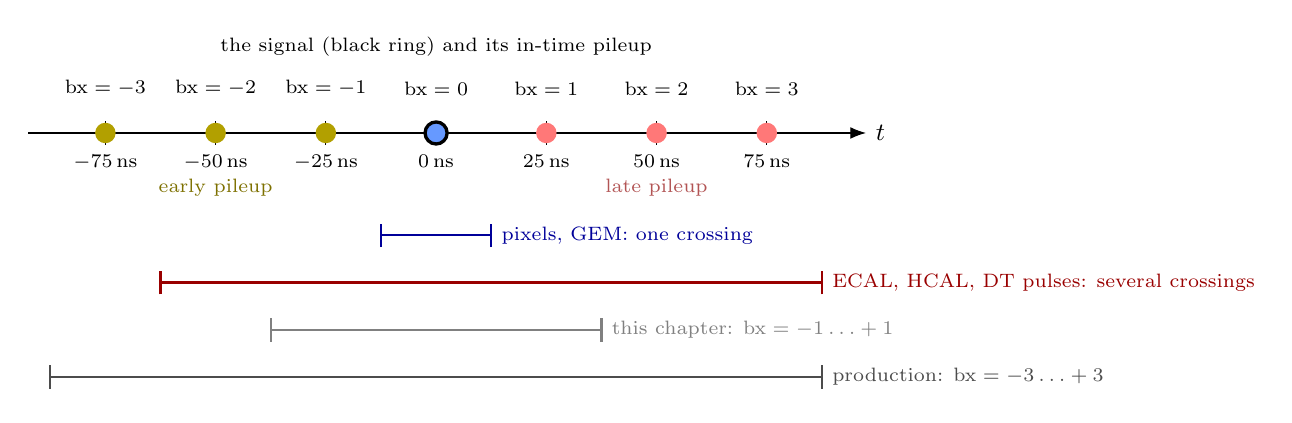
\begin{tikzpicture}[x=14mm, y=1mm, font=\small]
  \draw[-{Latex[length=2mm]}] (-3.7,0) -- (3.9,0) node[right] {$t$};
  \foreach \b/\t in {-3/-75,-2/-50,-1/-25,0/0,1/25,2/50,3/75} {
    \draw (\b,-1.5) -- (\b,1.5);
    \node[below, font=\scriptsize] at (\b,-1.5) {$\t\ns$};
    \node[above=2mm, font=\scriptsize] at (\b,1.5) {$\bx=\b$};
  }
  \fill[puearly] (-3,0) circle (1.3mm); \fill[puearly] (-2,0) circle (1.3mm); \fill[puearly] (-1,0) circle (1.3mm);
  \fill[puintime] (0,0) circle (1.3mm);
  \fill[pulate] (1,0) circle (1.3mm); \fill[pulate] (2,0) circle (1.3mm); \fill[pulate] (3,0) circle (1.3mm);
  \draw[very thick] (0,0) circle (1.4mm);
  \node[above=7mm, font=\scriptsize] at (0,1.5) {the signal (black ring) and its in-time pileup};
  \node[font=\scriptsize, text=puearly!70!black] at (-2,-7) {early pileup};
  \node[font=\scriptsize, text=pulate!70!black] at (2,-7) {late pileup};
  \draw[thick, blue!60!black] (-0.5,-13) -- (0.5,-13) node[right, font=\scriptsize] {pixels, GEM: one crossing};
  \draw[thick, blue!60!black] (-0.5,-14.5) -- (-0.5,-11.5); \draw[thick, blue!60!black] (0.5,-14.5) -- (0.5,-11.5);
  \draw[thick, red!60!black] (-2.5,-19) -- (3.5,-19) node[right, font=\scriptsize] {ECAL, HCAL, DT pulses: several crossings};
  \draw[thick, red!60!black] (-2.5,-20.5) -- (-2.5,-17.5); \draw[thick, red!60!black] (3.5,-20.5) -- (3.5,-17.5);
  \draw[thick, gray] (-1.5,-25) -- (1.5,-25) node[right, font=\scriptsize] {this chapter: $\bx=-1\ldots+1$};
  \draw[thick, gray] (-1.5,-26.5) -- (-1.5,-23.5); \draw[thick, gray] (1.5,-26.5) -- (1.5,-23.5);
  \draw[thick, gray!60!black] (-3.5,-31) -- (3.5,-31) node[right, font=\scriptsize] {production: $\bx=-3\ldots+3$};
  \draw[thick, gray!60!black] (-3.5,-32.5) -- (-3.5,-29.5); \draw[thick, gray!60!black] (3.5,-32.5) -- (3.5,-29.5);
\end{tikzpicture}
\caption{The time line of one triggered event. Bunches cross every $25\ns$; the signal sits in $\bx=0$ with
its in-time pileup, the crossings before and after carry the early and the late pileup. A detector whose
readout window covers one crossing sees only $\bx=0$; a detector whose signal lasts longer than $25\ns$
integrates the neighbouring crossings too. The simulation therefore overlays pileup on a window of
crossings: $-1\ldots+1$ in this chapter, $-3\ldots+3$ in the production.}
\label{fig:timeline}
\end{figure}

\begin{plainwords}
Think of a long-exposure photograph of a street at night. A camera with a fast shutter captures one
instant: only the cars that are in the frame at that moment (the in-time pileup). A camera with a slow
shutter also records the cars that passed shortly before and after, as streaks (the out-of-time pileup).
The detectors of CMS have different shutter speeds: the pixels are fast, the calorimeter pulses are slow.
The simulation has to provide the ``cars'' of the neighbouring instants too, which is why it mixes pileup
into a window of bunch crossings rather than into one.
\end{plainwords}

\paragraph{Why it matters.} Pileup adds hits, energy and vertices that have nothing to do with the hard
scattering: it degrades the jet energy resolution, fakes jets and missing energy, creates spurious tracks and
vertices, increases occupancy and data volume, and ages the detectors. Everything downstream (the pixel and
strip cluster thresholds, the HGCal and MTD timing, the vertex finding, the pileup-per-particle identification
in the particle flow, the jet energy corrections, the pileup jet id) is designed against it. This chapter is
where one sees the raw material those algorithms have to work with.

% ======================================================================================================
\section{How CMSSW simulates pileup}
\label{sec:how}

The simulation chain for one signal event is GEN $\to$ SIM $\to$ DIGI $\to$ \ldots{}. Pileup enters in the
DIGI step, i.e.\ after Geant4 and before the detector electronics, by \emph{mixing}: the minimum-bias events
are simulated once and for all, as a library, and the \code{MixingModule} overlays a random selection of
them on every signal event before the digitisers run. Figure~\ref{fig:flow} shows the data flow as it is
realised in this chapter.

\begin{plainwords}[Why the pileup is added after Geant4 and not before]
Geant4 is by far the most expensive step of the chain (seconds per event, section~\ref{sec:library}), and
the hits it produces are \emph{additive}: a sensor crossed by a signal particle and by a pileup particle
simply holds two hits, and a calorimeter cell holds the sum of the two energies. So nothing is lost by
simulating every collision separately and adding the hits afterwards, and a great deal is gained: a
minimum-bias event simulated once can be overlaid on thousands of different signal events. Overlaying
\emph{before} Geant4 (putting the particles of all the collisions into one Geant4 event) would be physically
equivalent, but would cost the full Geant4 time of $\sim1400$ events for every single signal event.
\end{plainwords}

\begin{figure}[H]
\centering
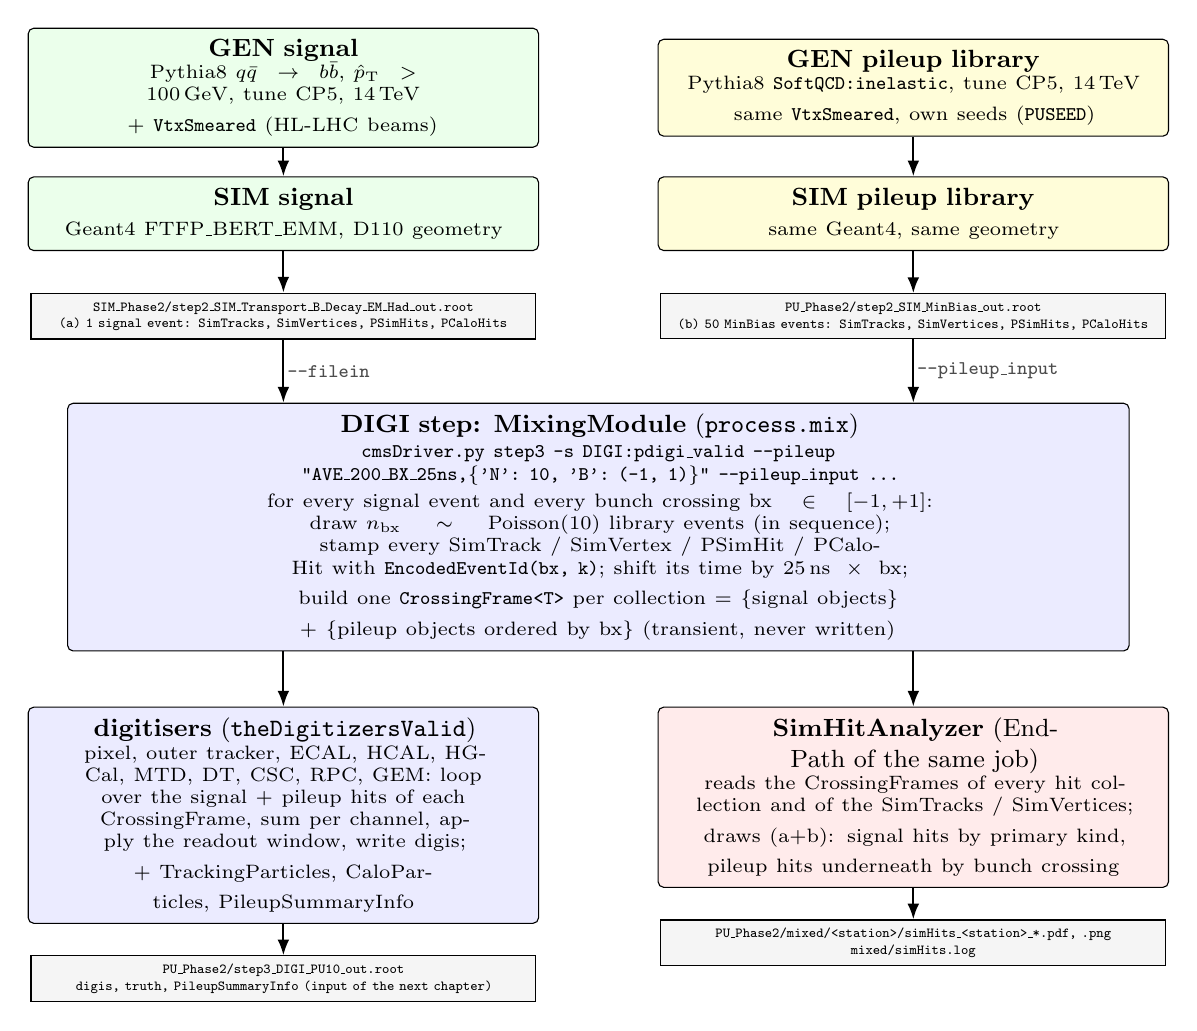
\begin{tikzpicture}[
  box/.style={draw, rounded corners=2pt, align=center, font=\small, minimum height=8mm, inner sep=4pt, fill=white},
  file/.style={draw, align=center, font=\tiny\ttfamily, inner sep=3pt, fill=gray!8},
  arr/.style={-{Latex[length=2mm]}, thick},
  lab/.style={font=\scriptsize\ttfamily, text=gray!60!black, fill=white, inner sep=1pt},
]
% signal column (x = 0) and pileup column (x = 8 cm)
\node[box, fill=green!8, text width=62mm] (sgen) at (0,0) {\textbf{GEN signal}\\\scriptsize Pythia8 $q\bar q\to\bbbar$, $\ptHat>100$\,GeV, tune CP5, 14\,TeV\\\scriptsize + \code{VtxSmeared} (HL-LHC beams)};
\node[box, fill=green!8, text width=62mm] (ssim) at (0,-1.6) {\textbf{SIM signal}\\\scriptsize Geant4 FTFP\_BERT\_EMM, D110 geometry};
\node[file, text width=62mm] (sfile) at (0,-2.9) {SIM\_Phase2/step2\_SIM\_Transport\_B\_Decay\_EM\_Had\_out.root\\(a) 1 signal event: SimTracks, SimVertices, PSimHits, PCaloHits};
\node[box, fill=yellow!15, text width=62mm] (pgen) at (8,0) {\textbf{GEN pileup library}\\\scriptsize Pythia8 \code{SoftQCD:inelastic}, tune CP5, 14\,TeV\\\scriptsize same \code{VtxSmeared}, own seeds (\code{PUSEED})};
\node[box, fill=yellow!15, text width=62mm] (psim) at (8,-1.6) {\textbf{SIM pileup library}\\\scriptsize same Geant4, same geometry};
\node[file, text width=62mm] (pfile) at (8,-2.9) {PU\_Phase2/step2\_SIM\_MinBias\_out.root\\(b) 50 MinBias events: SimTracks, SimVertices, PSimHits, PCaloHits};
% mixing
\node[box, fill=blue!8, text width=132mm, anchor=north] (mix) at (4,-4.0)
  {\textbf{DIGI step: MixingModule} (\code{process.mix})\\[1pt]
   \scriptsize\code{cmsDriver.py step3 -s DIGI:pdigi\_valid --pileup "AVE\_200\_BX\_25ns,\{'N': 10, 'B': (-1, 1)\}" --pileup\_input ...}\\[2pt]
   \scriptsize for every signal event and every bunch crossing $\bx\in[-1,+1]$: draw $n_{\bx}\sim\mathrm{Poisson}(10)$ library events (in sequence);\\
   \scriptsize stamp every SimTrack / SimVertex / PSimHit / PCaloHit with \code{EncodedEventId(bx, k)}; shift its time by $25\ns\times\bx$;\\
   \scriptsize build one \code{CrossingFrame<T>} per collection = \{signal objects\} + \{pileup objects ordered by bx\} (transient, never written)};
\node[box, fill=blue!8, text width=62mm, anchor=north] (digi) at ($(mix.south)+(-4,-0.7)$)
  {\textbf{digitisers} (\code{theDigitizersValid})\\\scriptsize pixel, outer tracker, ECAL, HCAL, HGCal, MTD, DT, CSC, RPC, GEM: loop over the signal + pileup hits of each CrossingFrame, sum per channel, apply the readout window, write digis;\\\scriptsize + TrackingParticles, CaloParticles, PileupSummaryInfo};
\node[box, fill=red!8, text width=62mm, anchor=north] (ana) at ($(mix.south)+(4,-0.7)$)
  {\textbf{SimHitAnalyzer} (EndPath of the same job)\\\scriptsize reads the CrossingFrames of every hit collection and of the SimTracks / SimVertices;\\\scriptsize draws (a+b): signal hits by primary kind, pileup hits underneath by bunch crossing};
\node[file, text width=62mm, below=4mm of digi] (dfile) {PU\_Phase2/step3\_DIGI\_PU10\_out.root\\digis, truth, PileupSummaryInfo (input of the next chapter)};
\node[file, text width=62mm, below=4mm of ana] (afile) {PU\_Phase2/mixed/<station>/simHits\_<station>\_*.pdf, .png\\mixed/simHits.log};
% arrows
\draw[arr] (sgen) -- (ssim); \draw[arr] (ssim) -- (sfile);
\draw[arr] (pgen) -- (psim); \draw[arr] (psim) -- (pfile);
\draw[arr] (sfile.south) -- (sfile.south |- mix.north) node[lab, midway, right] {--filein};
\draw[arr] (pfile.south) -- (pfile.south |- mix.north) node[lab, midway, right] {--pileup\_input};
\draw[arr] (digi.north |- mix.south) -- (digi.north);
\draw[arr] (ana.north |- mix.south) -- (ana.north);
\draw[arr] (digi) -- (dfile); \draw[arr] (ana) -- (afile);
\end{tikzpicture}
\caption{Data flow of the pileup exercise as run by \code{runPileup\_mcPhase2\_BBbar.sh}. The signal and the
pileup library go through the same GEN (vertex smearing) and SIM (Geant4) configurations; they meet in the
DIGI step inside the \code{MixingModule}, whose transient \code{CrossingFrame}s feed both the digitisers and,
in this exercise, the \code{SimHitAnalyzer} that draws the pages of case (a+b). Cases (a) and (b) are drawn
from the two SIM files with the ordinary \code{simHitAnalyzer\_cfg.py}.}
\label{fig:flow}
\end{figure}

\subsection{The pileup library}
\label{sec:library}

The library is an ordinary GEN-SIM sample of minimum-bias events. In this chapter it is made by the script
with two \code{cmsDriver.py} steps, with the Run4D110 RelVal settings of the signal (conditions
\code{auto:phase2\_realistic\_T33}, era \code{Phase2C17I13M9}, geometry \code{ExtendedRun4D110}, beam spot
\code{DBrealisticHLLHC}):
\begin{lstlisting}[style=sh]
# (b) GEN: 50 minimum-bias events, HL-LHC vertex smearing, own random seeds
cmsDriver.py MinBias_14TeV_pythia8_TuneCP5_cfi --conditions auto:phase2_realistic_T33 --era Phase2C17I13M9 \
  --geometry ExtendedRun4D110 --beamspot DBrealisticHLLHC -n 50 -s GEN --datatier GEN --eventcontent FEVTDEBUG \
  --fileout file:step1_GEN_MinBias_out.root \
  --customise_commands "process.RandomNumberGeneratorService.generator.initialSeed = 20261\nprocess.RandomNumberGeneratorService.VtxSmeared.initialSeed = 20262"
# (b) SIM: the same Geant4 as the signal
cmsDriver.py step2 --filein file:step1_GEN_MinBias_out.root --conditions auto:phase2_realistic_T33 --era Phase2C17I13M9 \
  --geometry ExtendedRun4D110 --beamspot DBrealisticHLLHC -n -1 -s SIM --datatier GEN-SIM --eventcontent FEVTDEBUG \
  --fileout file:step2_SIM_MinBias_out.root \
  --customise_commands "process.RandomNumberGeneratorService.g4SimHits.initialSeed = 20263"
\end{lstlisting}

For a reader who has not written a \code{cmsDriver.py} command before: it is the tool that writes a complete
CMSSW configuration (a \code{\_cfg.py} file) from a few options and then, unless \code{--no\_exec} is given,
runs it. The options used in this chapter are:
\begin{center}\small
\begin{tabularx}{\textwidth}{>{\raggedright\arraybackslash}p{54mm}X}
\toprule
option & what it sets \\
\midrule
first argument (\code{MinBias\_14TeV\_\ldots\_cfi}, \code{step2}, \code{step3}) & the generator fragment to
  load (GEN step), or just a name for the configuration (later steps) \\
\code{-s GEN}, \code{-s SIM}, \code{-s DIGI:pdigi\_valid} & the step to run and, after the colon, the
  sequence to use for it \\
\code{--filein}, \code{--fileout} & input and output ROOT files \\
\code{-n 50}, \code{-n -1} & number of events to process ($-1$: all events of the input) \\
\code{--conditions auto:phase2\_realistic\_T33} & the global tag: alignment, calibrations, beam spot, \ldots{}
  read from the conditions database \\
\code{--era Phase2C17I13M9} & the set of \emph{era modifiers} that adapt every module to the Phase-2 detector
  (e.g.\ which HGCal collections to mix) \\
\code{--geometry ExtendedRun4D110} & the detector geometry (D110 is the current Phase-2 layout) \\
\code{--beamspot DBrealisticHLLHC} & the vertex-smearing model of the GEN step (HL-LHC beams, parameters
  from the database) \\
\code{--datatier}, \code{--eventcontent FEVTDEBUG} & how the output is labelled and which products it keeps
  (\code{FEVTDEBUG}: everything, including the SimHits) \\
\code{--pileup}, \code{--pileup\_input} & the mixing scenario and the library file (DIGI step only,
  section~\ref{sec:mixing}) \\
\code{--customise\_commands "..."} & Python lines appended verbatim to the end of the configuration
  (a literal \code{\textbackslash n} separates lines); the usual way to change one parameter \\
\bottomrule
\end{tabularx}
\end{center}
The generated configurations are kept (\code{step1\_GEN\_MinBias\_cfg.py}, \ldots, appendix~\ref{app:files})
and can be read, edited and re-run with \code{cmsRun} by hand; reading one of them next to the command that
produced it is the fastest way to learn what the options do.

{\sloppy The generator fragment, \path{Configuration/Generator/python/MinBias_14TeV_pythia8_TuneCP5_cfi.py},
is the one the Phase-2 RelVal and production pileup libraries use:\par}
\begin{lstlisting}[style=py]
generator = cms.EDFilter("Pythia8ConcurrentGeneratorFilter",
    crossSection = cms.untracked.double(71.39e+09),   # pb, metadata only
    comEnergy = cms.double(14000.0),
    PythiaParameters = cms.PSet(
        pythia8CommonSettingsBlock,                      # tau0Max = 10 mm, ... (what Geant4 decays)
        pythia8CP5SettingsBlock,                         # tune CP5: NNPDF3.1, MPI pT0Ref = 1.41, sigmaTot = 100.309 mb, ...
        processParameters = cms.vstring('SoftQCD:inelastic = on'),
        parameterSets = cms.vstring('pythia8CommonSettings', 'pythia8CP5Settings', 'processParameters')))
\end{lstlisting}
Three points deserve attention:
\begin{itemize}
\item \textbf{Same vertex smearing as the signal.} The \code{VtxSmeared} module runs in the GEN step, so the
  library events carry their primary vertex (position \emph{and} time) already. The \code{MixingModule} does
  not re-smear them; it only adds the bunch-crossing time offset. The library must therefore be made with the
  beam spot of the scenario it will be mixed into.
\item \textbf{Own random seeds.} The random numbers of CMSSW are pseudo-random: a given seed always produces
  the same sequence, which is what makes every job reproducible. \code{cmsDriver.py} writes the same default
  seeds into every configuration.
  Had the library been generated with the defaults, its event $k$ would have had exactly the vertex of signal
  event $k$ (same \code{VtxSmeared} seed, same sequence of random numbers), and the first mixed pileup event
  would have sat on top of the signal vertex. The script sets \code{PUSEED} (generator), \code{PUSEED+1}
  (vertex smearing) and \code{PUSEED+2} (Geant4).
\item \textbf{Same Geant4.} The SIM step of the library is the standard full-physics step
  (\code{FTFP\_BERT\_EMM}, the stage \code{Transport\_B\_Decay\_EM\_Had} of the SIM chapter), on the same
  D110 geometry: the pileup hits are of exactly the same nature as the signal hits (same sensitive detectors,
  same thresholds, same shower library for the HF).
\end{itemize}
Cost: at $\sim 1$\,s per event the GEN step of 50 events took about a minute, the SIM step about 3 minutes
(3.6\,s per minimum-bias event, against $\sim 4$\,s for a signal event, log timestamps of
\code{step2\_SIM\_MinBias\_out.log}). Note the size of the library against what is consumed: with
$\mathrm{PU}=10$ in three bunch crossings every signal event uses on average 30 library events, so a library of
50 serves barely two signal events when read in sequence (section~\ref{sec:extend}).

\subsection{The production way: premixing}
\label{sec:premix}

In this chapter the mixing is done from the SimHits (the ``classical'' mixing). It is the way in which the
hits of both the signal and the pileup can still be told apart and drawn, and it is what the
\code{MixingModule} was written for. It does not scale to $\mathrm{PU}=200$ in production: every signal event
would have to read $\sim 1400$ library events (section~\ref{sec:scaling}), i.e.\ tens of GB per signal event.
Since Run~2 the production therefore uses \emph{premixing}:
\begin{enumerate}
\item \textbf{Stage 1} (\code{premix\_stage1} modifier): the minimum-bias events are mixed among themselves
  at the target pileup and digitised once; the result is a library of \emph{digitised pileup events}
  (PREMIX data tier), one per signal event to come, with the pileup \code{SimTrack}s/\code{PSimHit}s kept in
  \code{PCrossingFrame} form only where the digitisers need them (\code{mixSH.pcrossingFrames}).
\item \textbf{Stage 2} (\code{premix\_stage2}): the signal event is digitised alone and the
  \code{PreMixingModule} adds, channel by channel, \emph{one} premixed event to it (in ADC units); the
  \code{PileupSummaryInfo} is copied from the premixed event.
\end{enumerate}
The physics is the same; only the bookkeeping differs (one pileup event read per signal event instead of
$\sim 1400$). The price is that in a premixed sample the pileup SimHits are not available any more, and the
pages of this chapter cannot be made. For the PU~200 numbers that the pages of this chapter extrapolate to,
section~\ref{sec:scaling}.

\begin{plainwords}
Classical mixing cooks every dish from raw ingredients: for each signal event it reads $\sim1400$
minimum-bias events and adds their hits one by one. Premixing prepares the ``pileup soup'' once: it mixes
and digitises 1400 minimum-bias events into one premixed event, stores a large pot of such events, and later
ladles exactly one of them onto each digitised signal event. This chapter uses the raw ingredients, because
only then can one still see which hit came from which collision.
\end{plainwords}

% ======================================================================================================
\section{The MixingModule}
\label{sec:mixing}

\subsection{Configuration: the \code{--pileup} option of \code{cmsDriver.py}}

The DIGI step with pileup is generated with
\begin{lstlisting}[style=sh]
cmsDriver.py step3 --filein file:SIM_Phase2/step2_SIM_Transport_B_Decay_EM_Had_out.root \
  --pileup "AVE_200_BX_25ns,{'N': 10, 'B': (-1, 1)}" --pileup_input file:PU_Phase2/step2_SIM_MinBias_out.root \
  --conditions auto:phase2_realistic_T33 --era Phase2C17I13M9 --geometry ExtendedRun4D110 \
  -n -1 -s DIGI:pdigi_valid --datatier GEN-SIM-DIGI --eventcontent FEVTDEBUG --fileout file:step3_DIGI_PU10_out.root \
  --customise_commands "process.mix.input.sequential = cms.untracked.bool(True)\n\
process.source.eventsToProcess = cms.untracked.VEventRange('1:1:1')\n\
from JitJetSW.Journey.simHitAnalyzer_cff import addSimHitAnalyzer; process = addSimHitAnalyzer(process, outputDir='mixed', ...)"
\end{lstlisting}
The \code{--pileup} argument names a \emph{mixing scenario} of
\path{Configuration/StandardSequences/python/Mixing.py} and optionally overrides its numbers:
\begin{lstlisting}[style=py]
addMixingScenario("AVE_200_BX_25ns", {'file': 'SimGeneral.MixingModule.mix_POISSON_average_cfi', 'BX': 25, 'B': (-3, 3), 'N': 200})
\end{lstlisting}
i.e.\ the Poisson mixing module with bunch spacing $25\ns$, window $\bx=-3\ldots3$ and mean 200; the override
\code{\{'N': 10, 'B': (-1, 1)\}} keeps the module and the bunch spacing and changes the mean and the window.
What \code{cmsDriver.py} writes into the configuration is:
\begin{lstlisting}[style=py]
process.load('SimGeneral.MixingModule.mix_POISSON_average_cfi')      # mix = MixingModule(digitizers, mixObjects, input)
process.mix.input.nbPileupEvents.averageNumber = cms.double(10.000000)  # Poisson mean per bunch crossing
process.mix.bunchspace = cms.int32(25)                                   # ns
process.mix.minBunch = cms.int32(-1)
process.mix.maxBunch = cms.int32(1)
process.mix.input.fileNames = cms.untracked.vstring(['file:.../step2_SIM_MinBias_out.root'])
process.mix.digitizers = cms.PSet(process.theDigitizersValid)
process.digitisation_step = cms.Path(process.pdigi_valid)
\end{lstlisting}
\code{pdigi\_valid} is the digitisation sequence of the RelVal workflows (in this release the same task as
\code{pdigi}, \code{Configuration/StandardSequences/python/Digi\_cff.py}): \code{generatorSmeared} (passed
through), the random-engine state producer, the \code{mix} module, the calorimeter and muon digi tasks that
run after it (\code{simEcalDigis} selective readout, \code{simHcalDigis} zero suppression, the trigger
primitives, \code{simMuonDTDigis}, CSC, RPC and GEM digis), \code{addPileupInfo}, and the pruning of the
\code{DigiSimLink}s. The tracker, ECAL, HCAL, HGCal and MTD digitisers and the truth producers are not
separate modules in a path: they are \emph{sub-components of the MixingModule}
(\code{process.mix.digitizers}), called by it once the \code{CrossingFrame}s of an event are complete, so that
the pileup never has to be stored. \code{theDigitizersValid} differs from \code{theDigitizers} only in the
truth: the plain set keeps the \code{TrackingParticle}s of the signal only (\code{signalOnlyTP = True}), the
\code{Valid} set those of the pileup too, which is what makes the per-event counts of
section~\ref{sec:truth} possible. The \code{sequential = True} customisation makes the secondary source read
the library in order, from its first event (section~\ref{sec:drawing}); the \code{VEventRange} restricts the job
to the one signal event that is drawn; the last line adds the analyzer (section~\ref{sec:analyzer}).

\begin{plainwords}[Modules, paths and the schedule]
A CMSSW job is a set of \emph{modules} (producers that add products to the event, analyzers that only read
them, filters, output modules) and a \emph{schedule} that says in which order they run for every event. A
\code{Path} is an ordered list of modules; an \code{EndPath} is a list that runs after all the paths, where
output modules and analyzers usually go. \code{process.mix} is one producer; the digitisers are not separate
modules but objects owned by it, so ``run the mixing'' and ``run the digitisers'' is one call. Reading
\code{step3\_DIGI\_PU10\_cfg.py} from the bottom (\code{process.schedule}) upward is the quickest way to see
what the job actually does.
\end{plainwords}

\subsection{What the module does, event by event}
\label{sec:drawing}

For every signal event the \code{MixingModule} (\code{SimGeneral/MixingModule/plugins/MixingModule.cc})
does the following.
\begin{enumerate}
\item \textbf{Draws the number of pileup events per bunch crossing.} For every bunch crossing from
  \code{minBunch} to \code{maxBunch} a number $n_{\bx}$ is drawn from a Poisson distribution with mean \code{averageNumber}
  (\code{type = 'poisson'} of the secondary source; other types exist: \code{fixed}, \code{histo}, and the
  \code{probFunction} used by the production to reproduce a luminosity profile). Here, with mean 10 in three
  bunch crossings: $n_{-1}=7$, $n_0=8$, $n_{+1}=3$, 18 events in total for an expectation of 30 (a low but
  legitimate draw, see the fluctuations paragraph of section~\ref{sec:what}).
  The drawn numbers are written per bunch crossing into the \code{PileupSummaryInfo} collection
  (\code{addPileupInfo}, section~\ref{sec:truth}).
\item \textbf{Reads the library events.} The secondary source (\code{EmbeddedRootSource}, class
  \code{edm::PileUp}) reads $n_{\bx}$ events from the files of \code{input.fileNames}. By default
  (\code{sequential = False}) it jumps to random positions of the library and reads from there, so that the
  same library can serve many signal events in many jobs; with \code{sequential = True} it starts at the first
  event and reads on. The bunch crossings are filled in order, from \code{minBunch} to \code{maxBunch}, so in
  this exercise the pileup events of the drawn signal event are simply the first 18 events of the file:
  library events 1--7 go to $\bx=-1$, 8--15 to $\bx=0$ and 16--18 to $\bx=+1$, and no event is used twice.
  The numbering printed in table~\ref{tab:mixedevents} restarts at 1 for every bunch crossing because it is
  the event number \emph{within the crossing} (next point): ``event 1 of $\bx=0$'' is library event 8.
\item \textbf{Stamps and shifts every object.} For every mixed collection and every pileup event $k$ of bunch
  crossing $\bx$, the \code{Adjuster} (\code{SimGeneral/MixingModule/plugins/Adjuster.cc}) sets on every
  \code{SimTrack}, \code{SimVertex}, \code{PSimHit} and \code{PCaloHit} the \code{EncodedEventId(bx, k)}
  (a 32-bit word: bunch crossing in the upper 16 bits, event number in the lower 16) and adds
  $\bx\times\code{bunchspace}$ to its time:
\begin{lstlisting}[style=cpp]
void doTheOffset(int bunchSpace, int bcr, std::vector<SimVertex>& simvertices, unsigned int evtNr, int vertexOffset, bool wrap) {
  int timeOffset = bcr * bunchSpace;
  EncodedEventId id(bcr, evtNr);
  for (auto& item : simvertices) { item.setEventId(id); item.setTof(item.position().t() + timeOffset); }
}
void doTheOffset(int bunchSpace, int bcr, std::vector<PCaloHit>& calohits, unsigned int evtNr, int vertexOffset, bool wrap) {
  int timeOffset = bcr * bunchSpace;
  EncodedEventId id(bcr, evtNr);
  for (auto& item : calohits) { item.setEventId(id); item.setTime(item.time() + timeOffset); }
}
\end{lstlisting}
  The signal keeps \code{EncodedEventId(0, 0)} and its times. For example the third library event read for
  $\bx=-1$ is stamped \code{EncodedEventId(-1, 3)}: its \code{bunchCrossing()} returns $-1$, its
  \code{event()} returns 3, and all its vertex and hit times are $25\ns$ earlier than Geant4 left them. The
  Geant4 track ids of the pileup events are
  \emph{not} renumbered: a track id is unique only within one event, so from the DIGI step on a simulated
  object is identified by the pair (event id, track id). This is what the \code{DigiSimLink}s, the
  \code{TrackingParticle}s and the \code{SimHitAnalyzer} use: track id 42 exists in the signal and, in
  general, in every one of the 18 pileup events, and only the pair (\code{EncodedEventId}, 42) names one
  particle. For the \code{PSimHit}s the \code{wrap} option
  (\code{WrapLongTimes} parameter of the module, off by default and here) folds the time of flight of very
  late hits back into one bunch crossing; so a pileup tracker hit of $\bx=-1$ simply has its time of flight
  minus 25\,ns.
\item \textbf{Builds the CrossingFrames.} Every mixed collection becomes one
  \code{CrossingFrame<T>}\footnote{\code{SimDataFormats/CrossingFrame/interface/CrossingFrame.h}: the
  signal as a list of pointers into the signal product, the pileup as a list of pointers into the pileup
  products with the offsets of every bunch crossing and every source; the \code{MixCollection<T>} iterator
  walks the two in order and tells for every element whether it is signal (\code{getTrigger()}) and in which
  bunch crossing it is (\code{bunch()}).} labelled \code{mix:g4SimHits<Collection>} (e.g.\
  \code{mix:g4SimHitsEcalHitsEB}, \code{mix:g4SimHits} for the SimTracks): one list of signal objects and one
  list of pileup objects, the latter ordered by bunch crossing and, within a crossing, by event. What is
  mixed is configured in \code{process.mix.mixObjects} (\code{SimGeneral/MixingModule/python/mixObjects\_cfi.py}):
  \code{mixSH} (the \code{PSimHit} collections of the tracker, the muon chambers and the MTD),
  \code{mixCH} (the \code{PCaloHit} collections of ECAL, HCAL, ZDC, Castor and, through the
  \code{phase2\_hgcal} era modifier, the three HGCal collections), \code{mixTracks}, \code{mixVertices} and
  \code{mixHepMC}. The \code{CrossingFrame}s are \emph{transient} products: they are built in memory,
  consumed by the digitisers in the same module call, and never written to the output file (``transient''
  means exactly that: the product lives in the memory of the running job and nowhere else, and
  \code{edmDumpEventContent} of the output file will not show it; this is why the analyzer of
  section~\ref{sec:analyzer} has to run inside the mixing job). Moreover by
  default they are only built where a consumer in the event needs them: the \code{crossingFrames} list of
  \code{mixSH} contains only the muon and MTD collections, \code{mixCH} none (the calorimeter digitisers take the
  hits directly from the \code{MixCollection}), and \code{makeCrossingFrame = False} for the tracks and
  vertices. The analyzer therefore has to switch them on (section~\ref{sec:analyzer}).
\item \textbf{Runs the digitisers.} Each digitiser of \code{process.mix.digitizers} (pixel and Phase-2 outer
  tracker, ECAL, HCAL, the three HGCal digitisers, the MTD, plus the truth producers) is called with the signal hits and then with the pileup hits of
  every bunch crossing. It adds the energies in the same channel, applies the detector response (pulse
  shape, time window, noise, thresholds, zero suppression) and writes the digis. Here the out-of-time pileup
  does its damage: a hit 25\,ns early or late lands in a different time sample of the ECAL / HCAL / HGCal
  pulse, in a different drift time of the DT, or outside the pixel window.
\item \textbf{Builds the truth} (section~\ref{sec:truth}) and writes the \code{PileupSummaryInfo}.
\end{enumerate}

\subsection{What is kept of the truth}
\label{sec:truth}

The DIGI file of the mixing job (\code{step3\_DIGI\_PU10\_out.root}, 7.2\,MB for one event with the
\code{FEVTDEBUG} content) contains, besides the digis and the untouched SIM products of the signal:
\begin{itemize}
\item \code{vector<PileupSummaryInfo> addPileupInfo}: one entry per bunch crossing of the window with the
  number of interactions drawn and the Poisson mean (``true'' number of interactions), plus the bunch
  spacing. For the drawn event:
  \begin{center}\small
  \begin{tabular}{crr}
  \toprule
  bunch crossing & \code{getPU\_NumInteractions()} & \code{getTrueNumInteractions()} \\
  \midrule
  $-1$ & 7 & 10.0 \\
  $0$  & 8 & 10.0 \\
  $+1$ & 3 & 10.0 \\
  \bottomrule
  \end{tabular}
  \end{center}
  This is the collection the pileup reweighting of an analysis reads (the true number of the in-time
  crossing), and the one the next chapter starts from.
\item \code{vector<TrackingParticle> mix:MergedTrackTruth} and the matching \code{TrackingVertex}s: one
  \code{TrackingParticle} per simulated charged (or decaying) particle above threshold, built from the
  \code{SimTrack}s and \code{SimVertex}s of the signal \emph{and} of every pileup event, each carrying its
  \code{EncodedEventId}. The drawn event has 4698 \code{TrackingParticle}s, 889 of the signal and 3809 of the
  18 pileup events (from 1 for the diffractive event 6 of $\bx=-1$ to 834 for event 7 of $\bx=-1$). A
  reconstructed track associated to a \code{TrackingParticle} with \code{eventId().bunchCrossing() != 0}
  is an out-of-time pileup track; with \code{bunchCrossing() == 0} and \code{event() != 0}, an in-time
  pileup track.
\item \code{vector<CaloParticle> mix:MergedCaloTruth} and \code{vector<SimCluster>}: the calorimeter truth
  (one \code{CaloParticle} per particle entering the calorimeter, with its \code{SimCluster}s of hits), 1220
  of them, 336 of the signal; and the MTD equivalents (\code{MergedMtdTruth}).
\item \code{DigiSimLink}s (\code{PixelDigiSimLink}, \code{StripDigiSimLink}, \code{DTDigiSimLink},
  \code{GEMDigiSimLink}, \ldots): channel by channel, the (event id, track id) pairs that contributed to a
  digi with their fraction of the charge.
\item \code{CrossingFramePlaybackInfoNew mix}: which library events (file, event number) were mixed in which
  bunch crossing, so that a later job can replay (\code{playback = True}) exactly the same mixing.
\end{itemize}
The pileup \code{SimTrack}s and hits themselves are \emph{not} written: after this step the only handles on
``which pileup event'' are the event ids carried by the truth objects and the links.

\begin{plainwords}[How to tell, after the DIGI step, where a simulated particle came from]
Every truth object carries its \code{EncodedEventId}, and two numbers answer the question:
\begin{center}\footnotesize
\begin{tabular}{ccl}
\toprule
\code{bunchCrossing()} & \code{event()} & origin \\
\midrule
$0$ & $0$ & the signal (hard-scattering) event \\
$0$ & $\geq1$ & in-time pileup, collision number \code{event()} of $\bx=0$ \\
$\neq0$ & $\geq1$ & out-of-time pileup of bunch crossing \code{bunchCrossing()} \\
\bottomrule
\end{tabular}
\end{center}
This is the rule the \code{SimHitAnalyzer} applies to colour the pages, and the rule a tracking or jet
validation applies to call a reconstructed object ``signal'', ``in-time PU'' or ``out-of-time PU''.
\end{plainwords}

% ======================================================================================================
\section{Drawing the mixed event: \code{SimHitAnalyzer} in CrossingFrame mode}
\label{sec:analyzer}

The pages of the SIM chapters are drawn by \code{plugins/SimHitAnalyzer.cc} from the \code{g4SimHits}
collections of a SIM file. To draw the mixed event the same analyzer runs \emph{inside} the mixing job,
because the \code{CrossingFrame}s exist nowhere else. The helper \code{addSimHitAnalyzer} of
\code{python/simHitAnalyzer\_cff.py} does the three things needed:
\begin{lstlisting}[style=py]
def addSimHitAnalyzer(process, outputDir, sampleLabel='', phase2=None, **kwargs):
    mo = process.mix.mixObjects
    mo.mixSH.crossingFrames = cms.untracked.vstring(*mo.mixSH.subdets.value())   # CrossingFrame for every PSimHit collection
    mo.mixCH.crossingFrames = cms.untracked.vstring(*mo.mixCH.subdets.value())   # ... and every PCaloHit collection
    mo.mixTracks.makeCrossingFrame = cms.untracked.bool(True)                     # ... and the SimTracks
    mo.mixVertices.makeCrossingFrame = cms.untracked.bool(True)                   # ... and the SimVertices
    process.simHitAnalyzer = simHitAnalyzer(outputDir, sampleLabel, phase2=phase2, crossingFrame=True, **kwargs)
    process.simHitAnalyzer_step = cms.EndPath(process.simHitAnalyzer)             # after the digitisation
    process.schedule.append(process.simHitAnalyzer_step)
    return process
\end{lstlisting}
With \code{crossingFrame = True} every input tag of the stations becomes the \code{CrossingFrame} product
(\code{mix:g4SimHitsEcalHitsEB} instead of \code{g4SimHits:EcalHitsEB}), and the analyzer:
\begin{itemize}
\item \textbf{Separates the events.} It walks the \code{SimTrack} and \code{SimVertex}
  \code{MixCollection}s and sorts the tracks and vertices into one \code{SimEvent} per
  \code{EncodedEventId}: the signal (\code{getTrigger()}), and one per mixed pileup event with its bunch
  crossing (\code{it.bunch()}). From these it prints the summary of table~\ref{tab:mixedevents}: events,
  primaries and \code{SimTrack}s per bunch-crossing class, and for every pileup event its primaries, tracks,
  vertices and the position and time of its primary vertex (where the $25\ns\times\bx$ shift is visible).
\item \textbf{Assigns the hits.} A signal hit (\code{getTrigger()}) is traced to its signal primary through
  the \code{SimVertex} parent links exactly as in the SIM chapter and coloured by the kind of that primary
  (charged hadron, neutral hadron, photon, $e^\pm$, $\mu^\pm$, other, no stored ancestor). A pileup hit is
  not traced to its primary: it is given one of three new ``kinds'' according to its bunch crossing,
  \textcolor{puearly}{\textbf{early}} ($\bx<0$, dark yellow), \textcolor{puintime}{\textbf{in-time}}
  ($\bx=0$, light blue) or \textcolor{pulate}{\textbf{late}} ($\bx>0$, salmon):
\begin{lstlisting}[style=cpp]
enum Kind { CHARGED_HADRON = 0, NEUTRAL_HADRON, PHOTON, ELECTRON, MUON, OTHER_KIND, UNASSIGNED, PU_EARLY, PU_INTIME, PU_LATE, NKIND };
static int pileupOwner(int bx) { return bx < 0 ? -2 : (bx == 0 ? -3 : -4); }   // owner codes of pileup hits
...
MixCollection<PSimHit> col(h.product());
for (auto it = col.begin(); it != col.end(); ++it)
  addPSimHit(*it, it.getTrigger() ? primOfTrackId((*it).trackId()) : pileupOwner(it.bunch()));
\end{lstlisting}
\item \textbf{Sums the calorimeter cells.} As in the SIM chapter a calorimeter cell is one marker whose
  size grows with the summed energy of all hits in it; the energy is also summed \emph{per owner} (signal
  primary, or pileup class), and the cell takes the colour of the owner with the largest share. A cell that
  turns from green in (a) to blue in (a+b) is therefore a cell of a signal photon in which the in-time
  pileup now deposits more than the photon. The counts ``cells dominated by the signal / by pileup'' of the
  logs and of table~\ref{tab:stations} come from this rule.
\item \textbf{Draws the pileup underneath.} The hits are partitioned so that the pileup hits are drawn
  first and the signal hits on top, with slightly smaller markers for the pileup tracker hits; the leading
  signal primaries of every kind are followed through the layers as before. The header of every (a+b) page
  states the number of mixed events per bunch crossing, how many of the hits are signal and pileup, and that
  the hits of $\bx<0$ / $\bx>0$ arrive $25\ns\times|\bx|$ before / after the signal.
\end{itemize}

\begin{plainwords}[How to read an (a+b) page]
Take figure~\ref{fig:trk}c as the example. The title names the station and the view. The lines under it say
how many hits are drawn and in which subdetectors, how many are signal and how many pileup, how many pileup
events went into each bunch crossing, and which signal primaries are \emph{followed} (their hits joined by a
line in time order, their calorimeter cells circled). The legend on the right lists every colour with its hit
count: the signal kinds first (charged hadron, neutral hadron, photon, $e^\pm$, \ldots, no stored ancestor),
then the three pileup classes. The grey dots are the detector elements, drawn so that an empty layer is
still visible. The box in the top right corner states the sample: (a+b), the PU and the window, that the
library was read in sequence. The same station is drawn in the three views ($r$--$z$, $x$--$y$,
$\eta$--$\phi$) on the three pages of \code{simHits\_<station>\_run1\_event1.pdf} and in one PNG per view. The
legend counts are the numbers of table~\ref{tab:stations}; checking one of them against the table is a good
first exercise.
\end{plainwords}
The analyzer is scheduled in an \code{EndPath} after the digitisation path, so the \code{CrossingFrame}s
are complete when it runs. Because the digitisers and the analyzer run in the same job, the DIGI job of one
signal event took 23 minutes here (log timestamps), almost all of it in the drawing of the six stations with
$\sim 60\,000$ tracker hits and $\sim 67\,000$ calorimeter cells each. The lines of the analyzer are
extracted from the DIGI log into \code{mixed/simHits.log} by the script.

% ======================================================================================================
\section{The three samples}
\label{sec:samples}

Everything is drawn on the same stations (TRK, ECAL, HCAL, HGCAL, MUON, ALL) with the same three views
($r$--$z$, $x$--$y$ of the barrel, $\eta$--$\phi$ from the primary vertex), so that the pages can be put side
by side:

\begin{center}\small
\begin{tabularx}{\textwidth}{llX}
\toprule
case & directory & what is in it \\
\midrule
(a) signal & \code{PU\_Phase2/signal/} & the \bbbar{} event through Geant4, exactly the page of the SIM chapter
  (\path{SIM_Phase2/step2_SIM_Transport_B_Decay_EM_Had_out.root}, event 1:1:1); 518 primaries handed to
  Geant4, 4284 \code{SimTrack}s, $\mathrm{PV}=(0.001, -0.000, 0.551)\cm$ \\
(b) pileup & \code{PU\_Phase2/pileup/} & one minimum-bias event of the library through the same Geant4
  (\code{step2\_SIM\_MinBias\_out.root}, event 1 of 50); 182 primaries, 1128 \code{SimTrack}s,
  $\mathrm{PV}=(-0.001, 0.000, 0.027)\cm$ \\
(a+b) signal + pileup & \code{PU\_Phase2/mixed/} & the signal event as the \code{MixingModule} hands it to
  the digitisers: its own hits plus the hits of the 18 minimum-bias events it put into the bunch crossings
  $-1$, $0$ and $+1$ (2691 pileup primaries, 19\,090 pileup \code{SimTrack}s) \\
\bottomrule
\end{tabularx}
\end{center}

\subsection{The mixed events}

\begin{table}[H]
\centering\small
\caption{The 18 library events mixed into signal event 1:1:1 (\code{mixed/simHits.log}), with the
primaries handed to Geant4, the \code{SimTrack}s and \code{SimVertex}s kept, and the position and time of
the primary vertex after the mixing. The event number restarts at 1 in every bunch crossing (it is the
\code{event()} field of the \code{EncodedEventId}); the library was read in sequence, so these are the
first 18 events of the file. The time of the vertex is the bunch-crossing offset $25\ns\times\bx$ added by
the \code{Adjuster}; the per-event collision time of the HL-LHC beam model ($\sigma_t\simeq190$\,ps) is
below the printed precision. Event 1 of $\bx=-1$ is the event drawn alone as case (b).}
\label{tab:mixedevents}
\begin{tabular}{ccrrrrr}
\toprule
$\bx$ & event & primaries & SimTracks & SimVertices & vertex $z$ [cm] & vertex $t$ [ns] \\
\midrule
$-1$ & 1 & 182 & 1128 &  642 &  $0.03$ & $-25.0$ \\
$-1$ & 2 &  41 &  298 &  171 & $-6.49$ & $-25.0$ \\
$-1$ & 3 & 196 & 1391 &  803 & $-3.02$ & $-25.0$ \\
$-1$ & 4 &  65 &  299 &  173 & $-0.48$ & $-25.0$ \\
$-1$ & 5 &   1 &    1 &    1 &  $3.55$ & $-25.0$ \\
$-1$ & 6 &   5 &    6 &    3 & $-1.31$ & $-25.0$ \\
$-1$ & 7 & 498 & 3987 & 2411 &  $2.79$ & $-25.0$ \\
\midrule
 $0$ & 1 & 120 & 1021 &  654 & $-11.13$ & $0.0$ \\
 $0$ & 2 & 614 & 4119 & 2528 &  $0.83$ & $0.0$ \\
 $0$ & 3 &   8 &   57 &   42 &  $1.97$ & $0.0$ \\
 $0$ & 4 &  87 &  601 &  419 &  $4.80$ & $0.0$ \\
 $0$ & 5 &  81 &  548 &  364 & $-0.03$ & $0.0$ \\
 $0$ & 6 &  70 &  403 &  232 & $15.14$ & $0.0$ \\
 $0$ & 7 & 238 & 1488 &  860 &  $5.75$ & $0.0$ \\
 $0$ & 8 & 244 & 2177 & 1393 &  $0.88$ & $0.0$ \\
\midrule
$+1$ & 1 & 178 &  998 &  562 & $-4.78$ & $25.0$ \\
$+1$ & 2 &  49 &  321 &  193 &  $3.82$ & $25.0$ \\
$+1$ & 3 &  14 &  247 &  203 &  $5.65$ & $25.0$ \\
\midrule
\multicolumn{2}{l}{early ($\bx<0$), 7 events} & 988 & \multicolumn{4}{l}{} \\
\multicolumn{2}{l}{in-time ($\bx=0$), 8 events} & 1462 & \multicolumn{4}{l}{} \\
\multicolumn{2}{l}{late ($\bx>0$), 3 events} & 241 & \multicolumn{4}{l}{} \\
\multicolumn{2}{l}{all 18 events} & 2691 & 19\,090 & & $-11.1\ldots+15.1$ & \\
\multicolumn{2}{l}{signal, for comparison} & 518 & 4284 & & $0.55$ & $0.0$ \\
\bottomrule
\end{tabular}
\end{table}

Three things to read from table~\ref{tab:mixedevents}. First, the spread of the minimum-bias events: from a
single-track diffractive event (event 5 of $\bx=-1$: one primary, a forward proton) to events with more
primaries than the hard \bbbar{} event (614 against 518). The mean over the 18 is 150 primaries per event,
and the fluctuations are such that one event (event 2 of $\bx=0$) carries a quarter of the in-time pileup.
Second, the vertices: the signal vertex is at $z=0.55\cm$, the pileup vertices between $-11$ and $+15\cm$, the
$\pm4.3\cm$ Gaussian of the HL-LHC luminous region. An in-time pileup track from a vertex 10\,cm away does not
point back to the signal vertex, which is how the vertex finder will later separate them; its time differs
from the signal by the vertex-time spread of the beams (tens to hundreds of ps), which is what the MTD
measures. Third, the time offsets: all vertices of a bunch crossing move by the same $25\ns\times\bx$; the
early and late events are indistinguishable from the in-time ones in space, only in time.

\subsection{Station by station}

\begin{table}[H]
\centering\small
\caption{Hits per station in the three cases (\code{signal/simHits.log}, \code{pileup/simHits.log},
\code{mixed/simHits.log}): \code{PSimHit}s for the tracker and the muon system, \code{PCaloHit}s for the
calorimeters with the number of hit cells in parentheses (ALL: \code{PSimHit}s + \code{PCaloHit}s, e.g.\ 9970 + 54\,582
for the signal). The
stations are TRK (inner and outer tracker), ECAL (EB + HGCal EE), HCAL (HB, HO, HF + HGCal HSi, HSc), HGCAL
(EE, HSi, HSc), MUON (DT, CSC, RPC, GEM). In (a+b) the pileup is split by bunch crossing (early / in-time /
late): tracker and muon hits, or calorimeter cells whose largest energy share is pileup of that class; the
next column counts the cells dominated by a signal primary and by pileup. The last column gives the signal
primaries that left at least one hit in (a) and that still own a tracker hit or dominate a cell in (a+b).}
\label{tab:stations}
\scriptsize
\setlength{\tabcolsep}{3pt}
\newcommand{\hd}[1]{\begin{tabular}[b]{@{}c@{}}#1\end{tabular}}
\begin{tabular}{lrrrccc}
\toprule
station & \hd{(a)\\signal} & \hd{(b)\\one PU event} & \hd{(a+b)\\signal + pileup} & \hd{(a+b) pileup\\early / in-time / late} & \hd{(a+b) cells\\signal- / pileup-dom.} & \hd{primaries\\(a) $\to$ (a+b)} \\
\midrule
TRK   & 9940 & 3439 & 59\,685 & 19\,170 / 27\,076 / 3499 & -- & 307 $\to$ 307 \\
ECAL  & 50\,179 (12\,476) & 15\,156 (4713) & 275\,466 (60\,604) & 19\,083 / 26\,204 / 3876 & 11\,441 / 49\,163 & 323 $\to$ 321 \\
HCAL  & 4403 (2099) & 655 (515) & 12\,126 (6594) & 1905 / 2414 / 401 & 1874 / 4720 & 206 $\to$ 168 \\
HGCAL & 14\,817 (8936) & 4652 (3225) & 64\,275 (42\,159) & 12\,473 / 17\,796 / 3030 & 8860 / 33\,299 & 214 $\to$ 214 \\
MUON  & 30 & 24 & 150 & 53 / 59 / 8 & -- & 1 $\to$ 1 \\
ALL   & 64\,552 (14\,575) & 19\,274 (5228) & 347\,427 (67\,198) & 40\,211 / 55\,753 / 7784 & 13\,315 / 53\,883 & 476 $\to$ 462 \\
\bottomrule
\end{tabular}
\end{table}

\begin{table}[H]
\centering\small
\caption{Energy per station and per owner in (a+b) (\code{mixed/simHits.log}, ``hits by kind of the
primary''): the summed \code{PCaloHit} energy of the cells owned by signal primaries of each kind and by the
three pileup classes, in GeV, with the number of cells in parentheses. The HF numbers are in shower-library
units (photo-electrons), not GeV, which is why the HCAL row dwarfs the others; the HGCal numbers are the
energy deposited in the active silicon / scintillator (a few MeV per MIP), not the calibrated shower energy.
The signal energies are those of case (a) to within the cells that pileup took over.}
\label{tab:energy}
\setlength{\tabcolsep}{4pt}
\begin{tabular}{lrrrrrr}
\toprule
station & \textcolor{sigchg}{charged hadron} & \textcolor{signeu}{neutral hadron} & \textcolor{sigpho}{photon} & \textcolor{puearly}{pileup early} & \textcolor{puintime}{pileup in-time} & \textcolor{pulate}{pileup late} \\
\midrule
ECAL   & 24.6 (5048) & 6.65 (1747) & 22.2 (4129) & 123 (19\,083) & 129 (26\,204) & 11.2 (3876) \\
HCAL   & 985 (1020)  & 151 (799)   & 71 (48)     & 1330 (1905)   & 2510 (2414)   & 364 (401) \\
HGCAL  & 0.905 (4016) & 0.375 (2055) & 0.542 (2768) & 2.20 (12\,473) & 3.09 (17\,796) & 0.468 (3030) \\
\bottomrule
\end{tabular}
\end{table}

\paragraph{How to read tables~\ref{tab:stations} and~\ref{tab:energy}.} A few things that are easy to misread
the first time:
\begin{itemize}
\item \textbf{Hits add up, cells do not.} Tracker and muon hits are independent objects, so the (a+b) count is
  exactly the signal count plus the three pileup counts: $9940 + 19\,170 + 27\,076 + 3499 = 59\,685$ in the
  TRK row. A calorimeter cell, on the other hand, is hit by several collisions at once and is counted once,
  under its owner: the cells of (a+b) are fewer than the cells of (a) plus 18 times the cells of (b), and the
  signal-dominated cells of (a+b) (11\,441 in the ECAL) are fewer than the cells of (a) (12\,476), because
  about a thousand cells of the signal are now owned by pileup.
\item \textbf{The pileup columns are per class, not per event.} ``19\,083 / 26\,204 / 3876'' are the cells
  owned by all 7 early, all 8 in-time and all 3 late events together; per collision that is roughly 2700 ECAL
  cells (section~\ref{sec:scaling}).
\item \textbf{Case (b) is one event, not the average.} Library event 1 (182 primaries) is on the large side of
  the 18 (mean 150); the single-primary event 5 of $\bx=-1$ would give an almost empty page.
\item \textbf{The stations overlap on purpose.} ECAL contains the HGCal EE and HCAL contains the HGCal HSi and
  HSc, because the stations group by function (electromagnetic / hadronic), while HGCAL shows the endcap
  calorimeter alone; the ALL station counts every subdetector once.
\item \textbf{Energies are in different units.} The EB energy is in GeV, the HF in shower-library units
  (photo-electrons), the HGCal in energy deposited in the active layers (MeV per crossing particle). Compare
  numbers within a row of table~\ref{tab:energy}, not between rows.
\end{itemize}

The pileup, at $\mathrm{PU}=10$ in three bunch crossings (30 expected, 18 drawn collisions, i.e.\ 2\,\% of
the production scenario), already outnumbers the hard-scattering event in every station: five to one in the
tracker, five to one in calorimeter cells, and in the HCAL and HGCal also in energy. Yet, as the pages show,
the signal is not destroyed: it is a dense, hard, collimated object (two $b$ jets at $\eta\simeq-1.5$ and a
forward system beyond $\eta=-3$) while the pileup is diffuse and soft. The following pages show how this looks
in each station; every figure puts the three cases together.

% ----------------------------------------------------------------------------------------------------
\FloatBarrier
\subsection{Tracker}

\begin{figure}[H]
\centering
\begin{subfigure}[t]{0.49\textwidth}
  \includegraphics[width=\linewidth]{signal/TRK/simHits_TRK_rz_run1_event1.png}
  \caption{(a) the signal: 9940 PSimHits of 307 primaries.}
\end{subfigure}\hfill
\begin{subfigure}[t]{0.49\textwidth}
  \includegraphics[width=\linewidth]{pileup/TRK/simHits_TRK_rz_run1_event1.png}
  \caption{(b) one minimum-bias event: 3439 PSimHits of 98 primaries.}
\end{subfigure}\\[4pt]
\begin{subfigure}[t]{0.49\textwidth}
  \includegraphics[width=\linewidth]{mixed/TRK/simHits_TRK_rz_run1_event1.png}
  \caption{(a+b) the signal + 18 pileup events: 59\,685 PSimHits, 49\,745 of them pileup.}
\end{subfigure}\hfill
\begin{subfigure}[t]{0.49\textwidth}
  \includegraphics[width=\linewidth]{mixed/TRK/simHits_TRK_xy_run1_event1.png}
  \caption{(a+b) transverse view of the barrel: 21\,013 hits in the barrel layers.}
\end{subfigure}
\caption{The tracker station (inner pixel barrel and disks, outer tracker barrel and disks of the Phase-2
tracker). In (a+b) the signal hits keep the colours of (a) (by kind of the primary), the pileup hits are drawn
underneath in dark yellow (early), light blue (in-time) and salmon (late).}
\label{fig:trk}
\end{figure}

The pileup hits outnumber the signal hits five to one, although the signal is a hard event and every pileup
event is soft: the tracker counts crossings, not energy, and 18 events with 2691 primaries simply cross more
sensors than one with 518. Pileup adds hits everywhere, with no structure in $\phi$ (figure~\ref{fig:trk}d);
in $r$--$z$ it fills every layer uniformly, the forward disks slightly more (the minimum-bias events are
forward). The signal $b$ jets are still visible as the dense black / purple / green bundles at
$\eta\simeq-1.5$ (negative $z$, $r$ up to the outer layers) and the forward particles beyond $\eta=-3$ in the
disks; in $x$--$y$ as the curved bundles of tracks of the first layers. At the SimHit level the three bunch
crossings sit exactly on top of each other: only the time distinguishes them. The pixel readout window and the
outer-tracker time stamping will later drop most of the early and late hits (19\,170 and 3499 of the 49\,745
pileup hits), the in-time ones (27\,076) stay. The $x$--$y$ view of the first pixel layers shows how the
in-time pileup tracks come from vertices spread along $z$ and therefore do not point back to the signal
vertex in $r$--$z$, which is what the primary-vertex finder exploits. The three followed signal primaries
($\Sigma^-$ 19.9\,GeV at $\eta=-3.77$, $K^0_S$ 5.7\,GeV, $\gamma$ 5.0\,GeV, converted) are found with the same
hits in (a) and (a+b): the tracker hits of the signal are untouched by the mixing, they are only accompanied.

% ----------------------------------------------------------------------------------------------------
\FloatBarrier
\subsection{Electromagnetic calorimeter}

\begin{figure}[H]
\centering
\begin{subfigure}[t]{0.49\textwidth}
  \includegraphics[width=\linewidth]{signal/ECAL/simHits_ECAL_etaphi_run1_event1.png}
  \caption{(a) the signal: 12\,476 cells, 54\,GeV.}
\end{subfigure}\hfill
\begin{subfigure}[t]{0.49\textwidth}
  \includegraphics[width=\linewidth]{pileup/ECAL/simHits_ECAL_etaphi_run1_event1.png}
  \caption{(b) one minimum-bias event: 4713 cells, 17\,GeV.}
\end{subfigure}\\[4pt]
\begin{subfigure}[t]{0.49\textwidth}
  \includegraphics[width=\linewidth]{mixed/ECAL/simHits_ECAL_etaphi_run1_event1.png}
  \caption{(a+b): 60\,604 cells, 11\,441 of them signal-dominated.}
\end{subfigure}\hfill
\begin{subfigure}[t]{0.49\textwidth}
  \includegraphics[width=\linewidth]{mixed/ECAL/simHits_ECAL_rz_run1_event1.png}
  \caption{(a+b) in $r$--$z$: the EB ring at $r=130\cm$ and the HGCal EE disks at $|z|>320\cm$.}
\end{subfigure}
\caption{The ECAL station: the barrel crystals (EB, $|\eta|<1.48$) and the electromagnetic section of the
HGCal (EE, $1.5<|\eta|<3$), in $\eta$--$\phi$ from the signal vertex. Marker size is the summed energy of the
cell; the colour is that of the owner with the largest energy share. The gap at $|\eta|\simeq1.5$ is the
barrel--endcap transition.}
\label{fig:ecal}
\end{figure}

The EB barrel ring and the HGCal EE fill up with low-energy pileup cells. The energy scale tells the story
(table~\ref{tab:energy}): the signal deposits 54\,GeV in the ECAL station, the 18 pileup events 263\,GeV,
spread over five times more cells: it is a diffuse, almost uniform-in-$\phi$ sea of small markers. Only
11\,441 of the 60\,604 hit cells are dominated by the signal: the $b$-jet cores keep their colour (the
$K^-$ 18.1\,GeV, the $K^0_L$ 23.7\,GeV and the $\gamma$ 10.6\,GeV of the followed list are still found with
the same cells, circled, at $\eta\simeq-1.5$, $\phi\simeq-2$), while isolated low-energy signal cells (the
tails of the showers, the soft photons of the underlying event) are drowned: 323 signal primaries dominated
at least one cell in (a), 321 in (a+b). In the EB the crystal is large and the pileup energy per crystal is
a few MeV on average, far below the signal shower cores: the $b$ jets are easily visible by eye. In the HGCal EE the
cells are small ($\sim1\,\mathrm{cm}^2$) and the pileup occupies them one by one; only the energy (marker
size) distinguishes the jet.

% ----------------------------------------------------------------------------------------------------
\FloatBarrier
\subsection{Hadron calorimeter}

\begin{figure}[H]
\centering
\begin{subfigure}[t]{0.49\textwidth}
  \includegraphics[width=\linewidth]{signal/HCAL/simHits_HCAL_rz_run1_event1.png}
  \caption{(a) the signal: 2099 cells.}
\end{subfigure}\hfill
\begin{subfigure}[t]{0.49\textwidth}
  \includegraphics[width=\linewidth]{pileup/HCAL/simHits_HCAL_rz_run1_event1.png}
  \caption{(b) one minimum-bias event: 515 cells, mostly one forward hadron in the HF.}
\end{subfigure}\\[4pt]
\begin{subfigure}[t]{0.49\textwidth}
  \includegraphics[width=\linewidth]{mixed/HCAL/simHits_HCAL_rz_run1_event1.png}
  \caption{(a+b): 6594 cells, 4720 of them pileup-dominated.}
\end{subfigure}\hfill
\begin{subfigure}[t]{0.49\textwidth}
  \includegraphics[width=\linewidth]{mixed/HCAL/simHits_HCAL_etaphi_run1_event1.png}
  \caption{(a+b) in $\eta$--$\phi$: HB in $|\eta|<1.4$, HGCal H in $1.5<|\eta|<3$, HF beyond.}
\end{subfigure}
\caption{The HCAL station: the barrel (HB), the outer calorimeter (HO), the forward calorimeter (HF,
$3<|\eta|<5$, at $z=\pm11.3$\,m) and the hadronic section of the HGCal (silicon HSi and scintillator HSc).
The HF cell energies are in shower-library units.}
\label{fig:hcal}
\end{figure}

Here the pileup dominates even in energy, because the minimum-bias events are forward: most of their energy
is carried by the beam remnants and the diffractive systems at large $|\eta|$, where the HF (3 to 5 in $|\eta|$)
collects it. In the single library event (b) essentially all of the HCAL-station energy is in the HF (161 cells, 260
shower-library units, against 0.04\,GeV in 43 HB cells); in (a+b) the HF is the station with the largest pileup share, and in the HGCal hadronic part four cells out
of five are pileup-dominated. Of the 206 signal primaries that owned at least one HCAL cell in (a), 38 own
none in (a+b): the soft hadrons of the signal underlying event lose their cells to the pileup, and only the
jet cores (the $K^0_L$ of 23.7\,GeV, the charged hadrons of the $b$ jets at $\eta\simeq-1.5$ in the HGCal H and
the $\Sigma^-$ in the HF) remain signal-dominated. The HB is the quietest part (636 cells in (a+b) against 22\,777
in the EB): the barrel hadron calorimeter sees the pileup as a few hundred MeV per tower, which the
out-of-time part spreads over its time samples.

% ----------------------------------------------------------------------------------------------------
\FloatBarrier
\subsection{High-granularity endcap calorimeter}

\begin{figure}[H]
\centering
\begin{subfigure}[t]{0.49\textwidth}
  \includegraphics[width=\linewidth]{signal/HGCAL/simHits_HGCAL_etaphi_run1_event1.png}
  \caption{(a) the signal: 8936 cells.}
\end{subfigure}\hfill
\begin{subfigure}[t]{0.49\textwidth}
  \includegraphics[width=\linewidth]{pileup/HGCAL/simHits_HGCAL_etaphi_run1_event1.png}
  \caption{(b) one minimum-bias event: 3225 cells.}
\end{subfigure}\\[4pt]
\begin{subfigure}[t]{0.49\textwidth}
  \includegraphics[width=\linewidth]{mixed/HGCAL/simHits_HGCAL_etaphi_run1_event1.png}
  \caption{(a+b): 42\,159 cells, 33\,299 of them pileup-dominated.}
\end{subfigure}\hfill
\begin{subfigure}[t]{0.49\textwidth}
  \includegraphics[width=\linewidth]{mixed/HGCAL/simHits_HGCAL_rz_run1_event1.png}
  \caption{(a+b) in $r$--$z$: the 26 EE layers and the 21 hadronic layers of each endcap.}
\end{subfigure}
\caption{The HGCal station (EE, HSi, HSc) in $\eta$--$\phi$ and $r$--$z$. The $x$--$y$ view does not exist for
this station (no barrel). The crosses are the points where the signal primaries crossed the tracker /
calorimeter boundary.}
\label{fig:hgcal}
\end{figure}

The endcap calorimeter is where the HL-LHC pileup hurts most, and it is the reason the HGCal was built the
way it was: 33\,299 of the 42\,159 hit cells are pileup-dominated already at $\mathrm{PU}=10\times3$ bunch
crossings; the $\eta$--$\phi$ page of (a+b) is almost uniformly blue and yellow in $|\eta|>1.5$, with the
signal $b$ jet at $(\eta,\phi)\simeq(-1.5,-2.1)$ standing out only because of its energy (the large circled
cells of the $K^-$, $K^0_L$ and $\gamma$). Per layer (the ``hits by subdetector and layer'' line of the log)
the hit cells are concentrated in the first EE layers (2300--2900 cells in each of layers 1--7, 600 in layer
26, 500 in the first HSi layer, 20--50 in the last ones): the soft pileup particles shower early and stop,
while the signal jet reaches the hadronic layers. The numbers of
cells per bunch crossing (12\,473 early, 17\,796 in-time, 3030 late) are what the HGCal time-over-threshold
and time-of-arrival measurement of every cell (and the MTD for every track) is designed to separate: the
early and late pileup is 25\,ns away, the in-time pileup from vertices 1--15\,cm away is tens to hundreds of
picoseconds away, and the HGCal digitiser indeed applies a time window per cell in the next step. At
$\mathrm{PU}=200$ in seven bunch crossings the same pages would hold $\sim50$ times more pileup cells than
signal cells.

% ----------------------------------------------------------------------------------------------------
\FloatBarrier
\subsection{Muon system and all stations}

\begin{figure}[H]
\centering
\begin{subfigure}[t]{0.49\textwidth}
  \includegraphics[width=\linewidth]{mixed/MUON/simHits_MUON_rz_run1_event1.png}
  \caption{(a+b) muon station: 30 signal + 120 pileup PSimHits, all in the CSC and GEM forward stations.}
\end{subfigure}\hfill
\begin{subfigure}[t]{0.49\textwidth}
  \includegraphics[width=\linewidth]{mixed/MUON/simHits_MUON_etaphi_run1_event1.png}
  \caption{(a+b) muon station in $\eta$--$\phi$.}
\end{subfigure}\\[4pt]
\begin{subfigure}[t]{0.49\textwidth}
  \includegraphics[width=\linewidth]{signal/ALL/simHits_ALL_rz_run1_event1.png}
  \caption{(a) all stations, the signal alone.}
\end{subfigure}\hfill
\begin{subfigure}[t]{0.49\textwidth}
  \includegraphics[width=\linewidth]{mixed/ALL/simHits_ALL_rz_run1_event1.png}
  \caption{(a+b) all stations: 127\,033 drawn hits, 103\,748 of them pileup.}
\end{subfigure}
\caption{The muon station and the ALL station. In the muon system the pileup reaches only the forward
chambers (GE0 / GE1 and the first CSC stations) through punch-through of forward hadrons; no pileup muon in
these 18 events. The ALL page shows the whole detector from the pixels to the HF.}
\label{fig:muon}
\end{figure}

Pileup reaches the muon system only through punch-through and the forward stations: 120 pileup hits against
30 signal hits, 109 of the 150 in the innermost GEM station (GE0, $|\eta|$ up to 2.8) and 35 in the first two
CSC stations, none in the barrel drift tubes or RPCs: the pattern of punch-through of forward hadrons rather than of
muons (a minimum-bias event rarely produces a muon above the few GeV needed to reach the chambers, and 18
events are too few). In the production scenario,
with 80 times more pileup collisions, the forward muon chambers do see a sizable rate of punch-through and of
neutron-induced background, which is simulated separately (the neutron background is not part of the
minimum-bias library). The ALL page of (a+b) sums it up: 23\,285 drawn objects of the signal under 103\,748
of the pileup, the $b$ jets still the densest structures in the picture.

% ----------------------------------------------------------------------------------------------------
\FloatBarrier
\subsection{Questions to test yourself}
\label{sec:questions}

Each question can be answered from the tables and figures of this section; the answers are in the footnotes.
\begin{enumerate}
\item The tracker has 59\,685 hits in (a+b). How many of them will the pixel detector, with its one-crossing
  readout window, ideally keep?\footnote{The signal and the in-time pileup: $9940 + 27\,076 = 37\,016$; the
  19\,170 early and 3499 late hits fall outside the window.}
\item Why does the HF show more pileup energy than any other subdetector, although its cells are few and
  far from the collision point?\footnote{Minimum-bias collisions send most of their energy forward (beam
  remnants, diffractive systems) and the HF covers $3<|\eta|<5$; the shower-library units also inflate the
  numbers compared with the GeV of the other rows.}
\item Event 2 of $\bx=0$ has 614 primaries, more than the \bbbar{} signal (518). Is it a ``hard'' event?\footnote{Not
  necessarily: a non-diffractive minimum-bias event with many multiple-parton interactions can have many soft
  primaries. What makes the signal hard is the $\ptHat>100\GeV$ of its two $b$ jets, not its multiplicity.}
\item In the HGCal, 33\,299 of the 42\,159 cells are pileup-dominated. Which measurement, made in the next step,
  can separate the 15\,503 early and late ones from the rest?\footnote{The time of arrival of each cell: the
  early and late pileup is $25\ns$ away from the signal, far beyond the $\sim50$\,ps resolution of the HGCal
  cells; the in-time pileup is the hard part.}
\item If the library had 20 events instead of 50, what would have happened in this very mixing job?\footnote{Nothing
  yet, since 18 events were needed and read in sequence; with a slightly higher draw (say 22) the secondary
  source would have wrapped around and the same library event would appear twice with two event ids
  (section~\ref{sec:extend}).}
\item The signal vertex is at $z=0.55\cm$ and pileup event 6 of $\bx=0$ at $z=15.1\cm$. Which detector
  separates the two, and which one separates the signal from event 1 of $\bx=-1$ at $z=0.03\cm$?\footnote{The
  tracker's vertex finder separates vertices $15\cm$ apart along $z$; the event of $\bx=-1$ sits at nearly
  the same $z$ but $25\ns$ earlier, so only the time (pixel readout window, MTD, HGCal timing) separates it.}
\item Table~\ref{tab:stations} says 206 signal primaries owned an HCAL cell in (a) and 168 in (a+b). Did the
  mixing remove signal hits?\footnote{No: the signal hits are untouched (every signal \code{PCaloHit} is still
  there). 38 primaries lost the \emph{ownership} of their cells because a pileup particle deposited more energy
  in the same cell. The pages colour a cell by its largest contributor only.}
\end{enumerate}

% ======================================================================================================
\FloatBarrier
\section{From this exercise to the production scenario}
\label{sec:scaling}

The pages above show $\mathrm{PU}=10$ in $\bx=-1\ldots+1$, i.e.\ an expectation of 30 (18 drawn) collisions
per signal event. The Phase-2 production mixes $\mathrm{PU}=200$ in $\bx=-3\ldots+3$: $7\times200=1400$
collisions, 47 times the expectation of this exercise and 78 times what was drawn. Since the pileup hits add
linearly, table~\ref{tab:scaling} scales the numbers of the mixed event to the production scenario (per
collision: the 18 events of table~\ref{tab:mixedevents} give the mean, the single event (b) the spread).

\begin{table}[H]
\centering\small
\caption{Pileup per minimum-bias collision, averaged over the 18 mixed events, and the expectation for one
signal event in the production scenario ($1400$ collisions, of which 200 in-time). The signal column is the
\bbbar{} event of this chapter. The cell counts saturate (two collisions can hit the same cell), so the
production cell numbers are upper limits; the hit counts do not.}
\label{tab:scaling}
\footnotesize
\begin{tabular}{lrrrr}
\toprule
 & per PU collision & this exercise (18) & production (1400) & signal event \\
\midrule
primaries handed to Geant4 & 150 & 2691 & $2.1\times10^5$ & 518 \\
SimTracks & 1060 & 19\,090 & $1.5\times10^6$ & 4284 \\
TrackingParticles & 212 & 3809 & $3.0\times10^5$ & 889 \\
tracker PSimHits & 2764 & 49\,745 & $3.9\times10^6$ & 9940 \\
ECAL station cells (pileup-dominated) & 2731 & 49\,163 & $\lesssim 3.8\times10^6$ & 12\,476 \\
HGCal cells (of $6.1\times10^6$) & 1850 & 33\,299 & $\lesssim 2.6\times10^6$ & 8936 \\
muon PSimHits & 6.7 & 120 & $9\times10^3$ & 30 \\
ECAL station energy & 14.6\,GeV & 263\,GeV & $20$\,TeV & 54\,GeV \\
\bottomrule
\end{tabular}
\end{table}

\begin{plainwords}[The arithmetic of table~\ref{tab:scaling}]
Seven bunch crossings at $\mu=200$ give $7\times200 = 1400$ expected collisions per signal event, against
$3\times10 = 30$ expected (18 drawn) here: factors 47 and 78. The ``per PU collision'' column is the (a+b)
pileup count divided by 18 (tracker: $49\,745/18 = 2764$ hits) and the production column is that times 1400
($2764\times1400 = 3.9\times10^{6}$). The energy estimate of consequence (iii) below goes: $14.6\GeV$ of
ECAL-station energy per collision $\times1400 = 20$\,TeV, of which one seventh (the in-time crossing) is
$\sim3$\,TeV; a jet of area $0.5$ in $\eta$--$\phi$ covers $0.5/(2\pi\times6) = 1.3$\,\% of the
calorimeter's $|\eta|<3$ area, hence $\sim40\GeV$ of in-time pileup energy under it.
\end{plainwords}

Three consequences follow. (i) \emph{Memory and time.} A classical mixing job at PU~200 holds $\sim10^6$
\code{SimTrack}s and $\sim10^7$ hits per event in the \code{CrossingFrame}s and reads $\sim1400$ library
events ($\sim 0.4$\,MB each in GEN-SIM) per signal event: this is why the production premixes
(section~\ref{sec:premix}), and why \code{runPileup\_mcPhase2\_BBbar.sh} at $\mathrm{PU}=200$ would need a
library of several thousand events and hours per signal event. (ii) \emph{Occupancy.} In the HGCal the
production pileup would occupy, on average, a large fraction of the $6.1\times10^6$ cells per event in the
first layers; in the inner pixel layers the per-module occupancy is what fixes the readout bandwidth. (iii)
\emph{Energy.} About 20\,TeV of pileup energy in the ECAL station against 54\,GeV of signal is the scale of the
pileup subtraction the jet reconstruction has to do: for a jet of area $0.5$ in $\eta$--$\phi$ out of
$\sim 2\pi\times6$, the in-time share ($1/7$ of it, $\sim3$\,TeV) is $\sim 40$\,GeV of pileup under a
100\,GeV jet, before the time windows of the digitisers and the charged-hadron subtraction take their part.

% ======================================================================================================
\section{Reproducing and extending}
\label{sec:extend}

Everything in this chapter is produced by one script from an initialised \code{CMSSW\_15\_0\_5} environment:
\begin{lstlisting}[style=sh]
cd JitJetSW/Journey/test
./runPileup_mcPhase2_BBbar.sh      # (a), (b), (a+b) with PU = 10 in bx -1..1, library of 50 MinBias events, into PU_Phase2/
\end{lstlisting}
{\sloppy It builds the plugin if needed. If the signal SIM file does not exist it first calls the SIM script
of the book, \path{runCMSDrivers_mcPhase2_BBbar_SIM.sh}, for the stage \code{Transport\_B\_Decay\_EM\_Had}.
It then generates and simulates the library (reused if present, \code{REUSE=1}), runs the mixing job with
the analyzer inside, and draws the three cases. Its variables:\par}

\begin{center}\small
\begin{tabularx}{\textwidth}{>{\raggedright\arraybackslash}p{58mm}X}
\toprule
variable (default) & meaning \\
\midrule
\code{EVENT=1:1:1} & signal event drawn and mixed \\
\code{PU=10} & mean number of pileup events per bunch crossing (Poisson); production: 200 \\
\code{BUNCHES=-1,1} & bunch-crossing window \code{min,max}; production: \code{-3,3} \\
\code{PUEVENTS=50} & size of the library generated in (b); must cover $\mathrm{PU}\times n_{\bx}$ with margin, since the events are read in sequence \\
\code{PUEVENT=1} & library event drawn alone in (b) \\
\code{PUSEED=20261} & random-seed base of the library (generator, \code{VtxSmeared}, \code{g4SimHits} get \code{PUSEED}, $+1$, $+2$) \\
\code{SIGNAL\_INPUT=SIM\_Phase2/...} & the signal SIM file \\
\code{OUTDIR=PU\_Phase2} & output directory \\
\code{CASES="signal pileup mixed"} & subset of the cases \\
\code{STATIONS=TRK,ECAL} & subset of the stations (default all) \\
\code{HIGHLIGHT=1}, \code{HIGHLIGHT\_PTMIN=2}, \code{PNG=1}, \code{PRINTHITS=0} & analyzer options as in \code{runSimHitAnalyzer\_mcPhase2\_BBbar.sh} \\
\code{REUSE=1} & keep the existing library files (step1 GEN, step2 SIM); \code{REUSE=0} regenerates them. The
  mixing job (step3) and the drawings are always redone \\
\code{RUN=0} & only generate the \code{cmsDriver} configurations \\
\bottomrule
\end{tabularx}
\end{center}

Suggested variations, in increasing cost:
\begin{lstlisting}[style=sh]
PUEVENT=7 CASES=pileup ./runPileup_mcPhase2_BBbar.sh                     # draw the 498-primary library event alone
CASES=mixed PU=50 BUNCHES=0,0 PUEVENTS=100 ./runPileup_mcPhase2_BBbar.sh   # denser, in-time only pileup (no yellow / salmon)
CASES=mixed PU=10 BUNCHES=-3,3 PUEVENTS=120 ./runPileup_mcPhase2_BBbar.sh  # the production window, early pileup up to 75 ns
CASES=mixed PU=10 BUNCHES=-1,1 STATIONS=HGCAL,TRK EVENT=1:1:2 ./runPileup_mcPhase2_BBbar.sh  # another signal event
REUSE=0 PUSEED=777 ./runPileup_mcPhase2_BBbar.sh                          # a different library (and different mixed events)
\end{lstlisting}
When the library is too small for the requested \code{PU} and window, the secondary source wraps around
and reuses events: with \code{sequential = True} the same library event would then appear twice in the
mixed event with two event ids. Regenerate the library with a larger \code{PUEVENTS} (\code{REUSE=0}) instead.

\paragraph{Practical advice for a first run.}
\begin{itemize}
\item Run from a shell with the CMSSW environment set up (\code{cmsenv} in the \code{src} directory of
  the release); the script checks for it and stops with a message otherwise.
\item The full chain takes about half an hour: the library $\sim4$\,min, the mixing job with the drawing
  $\sim23$\,min, cases (a) and (b) a few minutes each. Run it in the background and keep the terminal output:
\begin{lstlisting}[style=sh]
nohup ./runPileup_mcPhase2_BBbar.sh > runPileup.nohup.log 2>&1 &
tail -f runPileup.nohup.log            # the script's progress lines; the cmsRun logs are in PU_Phase2/
\end{lstlisting}
  Do not edit the script while it is running (bash reads it incrementally).
\item \code{REUSE=1} (the default) reuses the library whatever \code{PU}, \code{BUNCHES} or \code{PUSEED} you
  set, so a new seed or a larger \code{PUEVENTS} needs \code{REUSE=0}. The DIGI output is named after
  \code{PU} only (\code{step3\_DIGI\_PU10\_out.root}): a run with another \code{BUNCHES} overwrites it.
\item If a step fails, read the \code{\_out.log} of that step in \code{PU\_Phase2/} (the script prints its
  last 80 lines) and the \code{.driver.log} of the \code{cmsDriver.py} call (appendix~\ref{app:files}).
\item Disk and memory: 50 library events are 19\,MB in GEN-SIM, so a library for $\mathrm{PU}=200$ in seven
  crossings (several thousand events) is a few GB, and the memory of the mixing job grows with the number of
  hits held in the \code{CrossingFrame}s. Increase \code{PU} in steps.
\end{itemize}

Things to look at beyond the pages:
\begin{itemize}
\item \code{mixed/simHits.log}: the list of mixed events (table~\ref{tab:mixedevents}) and, per station, the
  hits per subdetector and layer and per kind, with the energy per kind (table~\ref{tab:energy}).
\item The \code{PileupSummaryInfo} of \code{step3\_DIGI\_PU10\_out.root}, e.g.\ with FWLite:
\begin{lstlisting}[style=py]
from DataFormats.FWLite import Events, Handle
ev = Events('PU_Phase2/step3_DIGI_PU10_out.root'); h = Handle('std::vector<PileupSummaryInfo>')
for e in ev:
    e.getByLabel('addPileupInfo', h)
    for p in h.product(): print(p.getBunchCrossing(), p.getPU_NumInteractions(), p.getTrueNumInteractions())
\end{lstlisting}
\item The \code{TrackingParticle}s (\code{mix:MergedTrackTruth}) grouped by \code{eventId()}: the
  per-event counts of section~\ref{sec:truth} (889 signal, 3809 pileup) and the pileup vertex positions.
\item \code{edmDumpEventContent PU\_Phase2/step3\_DIGI\_PU10\_out.root}: what the DIGI step wrote (and that
  no \code{CrossingFrame} is in it).
\item The \code{--pileup} scenarios of \code{Configuration/StandardSequences/python/Mixing.py}, in
  particular the \code{probFunction} ones used by the production to follow a luminosity profile instead of a
  single Poisson mean.
\end{itemize}

The DIGI file of the mixing job holds the digis of the signal + pileup event and the
\code{PileupSummaryInfo} collection; it is the input of the next chapter, where the digitisers' time windows decide which of the hits drawn here
survive into the digis.

% ======================================================================================================
\appendix
\section{Files of \code{test/PU\_Phase2/}}
\label{app:files}

\begin{center}\small
\begin{tabularx}{\textwidth}{>{\hsize=1.25\hsize\raggedright\arraybackslash}X>{\hsize=0.75\hsize\raggedright\arraybackslash}X}
\toprule
file & content \\
\midrule
\code{step1\_GEN\_MinBias\_cfg.py}, \code{\_out.root} (2.0\,MB), \code{\_out.log} & (b) GEN of the 50-event library; \code{.driver.log}: the \code{cmsDriver.py} output \\
\code{step2\_SIM\_MinBias\_cfg.py}, \code{\_out.root} (19\,MB), \code{\_out.log} & (b) SIM of the library \\
\code{step3\_DIGI\_PU10\_cfg.py}, \code{\_out.root} (7.2\,MB), \code{\_out.log} & (a+b) mixing + digitisation of signal event 1:1:1; the log holds the analyzer printout \\
\code{signal/<station>/simHits\_<station>\_run1\_event1.pdf}, \code{\_<view>\_*.png} & (a), one PDF with the three views per station, plus one PNG per view; \code{signal/simHits.log} \\
\code{pileup/<station>/\ldots}, \code{pileup/simHits.log} & (b) \\
\code{mixed/<station>/\ldots}, \code{mixed/simHits.log} & (a+b); the log is the analyzer part of \code{step3\_DIGI\_PU10\_out.log} \\
\code{runPileup.log} & the script's own output: the summary lines of the three cases and the list of pages \\
\code{AtPileup.md} & the Markdown version of this chapter (\code{doc/sim/AtPileup.md}) \\
\bottomrule
\end{tabularx}
\end{center}

\section{Glossary}
\label{app:glossary}

\sloppy
\begin{description}[style=sameline,leftmargin=0pt,itemsep=2pt]
\item[hard scattering] the parton--parton collision with large momentum transfer that the generator was asked
  for (here $q\bar q\to\bbbar$ with $\ptHat>100\GeV$); the signal.
\item[soft collision] an inelastic collision with little transverse momentum, whose particles go mostly
  forward; what a minimum-bias event usually is.
\item[diffractive collision] an inelastic collision in which one or both protons survive or become a low-mass
  system, leaving a large rapidity gap; can be almost invisible in the central detector.
\item[instantaneous luminosity] $\mathcal{L}_{\mathrm{inst}}$, the collision rate per unit cross section
  (cm$^{-2}$s$^{-1}$); with the inelastic cross section and the bunch-crossing rate it gives $\mu$,
  eq.~(\ref{eq:mu}).
\item[Poisson distribution] the distribution of the number of independent events with a fixed mean $\mu$;
  standard deviation $\sqrt{\mu}$. The number of collisions per crossing follows it.
\item[pileup (PU)] the additional inelastic proton--proton collisions in the same (in-time) or neighbouring
  (out-of-time) bunch crossings as the hard scattering; also the mean number of them per crossing, $\mu$.
\item[bunch crossing (bx)] one crossing of two bunches, every 25\,ns; the signal is in $\bx=0$, $\bx<0$ is
  earlier, $\bx>0$ later.
\item[minimum bias] the inelastic collisions selected with the least possible bias (\code{SoftQCD:inelastic}
  in Pythia8: non-diffractive, single- and double-diffractive); the pileup library.
\item[pileup library] a GEN-SIM sample of minimum-bias events, simulated once and mixed many times.
\item[MixingModule] the \code{EDProducer} \code{mix} of the DIGI step that overlays a Poisson number of library
  events per bunch crossing on the signal and calls the digitisers.
\item[CrossingFrame$<$T$>$] the transient container of one mixed collection: the signal objects and the
  pileup objects of every bunch crossing; \code{MixCollection<T>} iterates over both.
\item[EncodedEventId] the (bunch crossing, event number) stamp on every mixed \code{SimTrack}, \code{SimVertex},
  \code{PSimHit}, \code{PCaloHit}, \code{TrackingParticle} and \code{CaloParticle}; $(0,0)$ is the signal.
\item[PileupSummaryInfo] per bunch crossing, the number of mixed collisions and the Poisson mean.
\item[premixing] the production scheme: the pileup is mixed and digitised once (stage 1) and one premixed
  event is added to each digitised signal event (stage 2).
\item[playback] a second mixing job that takes exactly the same library events as the first one, read back
  from its \code{CrossingFramePlaybackInfoNew} product.
\item[signal-dominated cell] in the pages of (a+b), a calorimeter cell in which a signal primary has the
  largest energy share; otherwise pileup-dominated.
\item[DIGI step, digitiser] the step that turns SimHits into the signals the electronics would record
  (digis: ADC counts, time samples); one digitiser per subdetector, here run inside the \code{MixingModule}.
\item[transient product] a product that exists only in the memory of the running job and is never written to
  the output file; the \code{CrossingFrame}s are transient.
\item[Path, EndPath, schedule] a \code{Path} is an ordered list of modules run for every event; an
  \code{EndPath} runs after all paths (output modules, analyzers); the schedule lists the paths of the job.
\item[TrackingParticle, CaloParticle] the truth objects built by the DIGI step for comparison with
  reconstructed tracks and calorimeter clusters: one per simulated particle, with its hits and its
  \code{EncodedEventId}; built for the signal and the pileup when \code{theDigitizersValid} is used.
\item[hit, cell] a hit is one \code{PSimHit} or \code{PCaloHit}; a cell is one calorimeter readout unit, in
  which several hits of several collisions add up.
\item[station] a group of subdetectors drawn on one \code{SimHitAnalyzer} page (TRK, ECAL, HCAL, HGCAL, MUON,
  ALL).
\item[owner] of a cell: the signal primary or the pileup class with the largest energy share in it; of a
  tracker hit: the primary it descends from or its pileup class.
\end{description}

\end{document}
